\documentclass{article}

%------------------------- packages -------------------------%
\usepackage[T1]{fontenc}
\usepackage[utf8]{vietnam}
\usepackage[unicode,hidelinks]{hyperref}    % for reference
\usepackage{geometry}   % for layout
\usepackage{amsmath}    % for math
\usepackage{xcolor}     % for color
% for figure
\usepackage{graphicx}
\usepackage{caption}    
% for code
\usepackage{minted}
% for table
\usepackage{float}      
\usepackage{paracol}
\usepackage{array}
\usepackage{multirow}
% for header & footer 
\usepackage{fancyhdr}
\usepackage{lastpage}
\usepackage{enumitem}
\usepackage{subcaption}
% \titleclass{\subsubsubsection}{straight}[\subsection]

%------------------------- set up -------------------------%
% figure
\graphicspath{{./images/}}              % path to image
\captionsetup[figure]{labelfont={small,bf,it},textfont={small,it}}
% paragraph
\setlength{\parindent}{0pt}
\setlength{\parskip}{4pt}               % disables indentation
\renewcommand{\baselinestretch}{1.5}    % line spacing
% color
\definecolor{codegreen}{rgb}{0,0.6,0}
\definecolor{codegray}{rgb}{0.5,0.5,0.5}
\definecolor{codepurple}{rgb}{0.58,0,0.82}
% code
\def\code#1{\texttt{#1}}    % font
\usemintedstyle{tango}         % minted theme
\setminted{
    % autogobble,             % remove all common leading whitespace
    baselinestretch=1.2,
    breaklines,
    % linenos,               % enables line numbers
    % fontsize=\footnotesize
}

%------------------------- layout & margin -------------------------%
\geometry{
    a4paper,        % redundant if already in \documentclass
    left=20.32mm,
    right=20.32mm,
    top=25.40mm,
    bottom=25.40mm,
    heightrounded,  % better use it
}

%------------------------- header & footer -------------------------%
\renewcommand{\headrulewidth}{0.5pt}
\renewcommand{\footrulewidth}{0.5pt}
\setlength{\headheight}{24.5pt}
\pagestyle{fancy}

\fancyhead{}    % clear all header fields
\fancyhead[L]{
    \begin{tabular}{ll}
        \begin{picture}(10,10)
            \put(0,-7){
\includegraphics[width=8mm]{hcmut.png}}
        \end{picture}&
    	\begin{tabular}{l}
    	    {\ttfamily Trường Đại học Bách Khoa Tp. Hồ Chí Minh} \\
    	    {\ttfamily Khoa Khoa học và Kỹ thuật Máy tính} \\
    	\end{tabular} 	
    \end{tabular}
}

\fancyfoot{}    % clear all footer fields
\fancyfoot[L]{\footnotesize {\ttfamily Hệ cơ sở dữ liệu (CO2014) - Học kì 221}}
\fancyfoot[R]{\footnotesize {\ttfamily Trang {\thepage}/\pageref{LastPage}}}
% might change to \scriptsize

%------------------------- body -------------------------%
\begin{document}

%-------------------- cover --------------------%
\begin{titlepage}
\begin{center}
    \large ĐẠI HỌC QUỐC GIA VIỆT NAM \\
    TRƯỜNG ĐẠI HỌC BÁCH KHOA TP. HỒ CHÍ MINH \\
    KHOA KHOA HỌC VÀ KỸ THUẬT MÁY TÍNH
\end{center}

\vspace{1.5cm}

\begin{figure}[!ht]
    \centering 
\includegraphics[width=3.5cm]{hcmut.png}
\end{figure}

\vspace{1.5cm}

\begin{table}[H]
    \centering
    \begin{tabular}{c}
    {\bf \Large HỆ CƠ SỞ DỮ LIỆU (CO2014)}    \\  \\
    \hline  \\
    \multicolumn{1}{l}{{\bf \large Báo cáo Bài tập lớn số 2}}    \\  \\
    {\bf \huge HỆ THỐNG ĐẶT VÉ PHIM}     \\  \\
    {\bf \huge ONLINE E-CINEMA} \\ \\
    \hline
    \end{tabular}
\end{table}

\vspace{1.5cm}

\begin{table}[H]
\centering
\begin{tabular}{lrlc}
\hspace{5.5 cm} & Giảng viên hướng dẫn: & Trương Quỳnh Chi    &          \\
                & Sinh viên thực hiện: & Võ Minh Duy   & 1910099  \\ 
                &                       &Trương Phi Trường     & 1915749   \\
                &                       & Phạm Lê Bảo & 2010153 \\
                &                       & Tiêu Thái Ngọc  & 2010455  \\
                &                       & Bùi Đoàn Gia Phong & 2010509  

\end{tabular}
\end{table}

\vspace{1.0cm}

\begin{center}
    \footnotesize Tp. Hồ Chí Minh, Tháng 12/2022
\end{center}
\end{titlepage}

%\renewcommand{\arraystretch}{2}

\newpage
%-------------------- contents --------------------%
\tableofcontents

\newpage
%-------------------- main --------------------%

\section{Tạo bảng và dữ liệu mẫu}
\subsection{Các câu lệnh tạo bảng và ràng buộc}
Bảng Admin và Customer:
\begin{minted}{mysql}
CREATE TABLE Admin (
	AdminID        VARCHAR(9)      PRIMARY KEY,
	Username       VARCHAR(50)     NOT NULL	UNIQUE,
	Password       VARCHAR(50)     NOT NULL,
	Name           VARCHAR(50)     NOT NULL,
	Birthday       DATE            NOT NULL,
	Gender         VARCHAR(50)     NOT NULL,
	Address        VARCHAR(50)     NOT NULL,
	Phone          VARCHAR(50)     NOT NULL,
	Email          VARCHAR(50)     NOT NULL,
	Created_time   DATETIME        NOT NULL,
	Certificate    VARCHAR(10)     NOT NULL
);
\end{minted}
\begin{minted}{mysql}
CREATE TABLE Customer (
        CustomerID     VARCHAR(9)      PRIMARY KEY,
	Username       VARCHAR(50)     NOT NULL            UNIQUE,
	Password       VARCHAR(50)     NOT NULL,
	Name           VARCHAR(50)     NOT NULL,
	Birthday       DATE            NOT NULL,
	Gender         VARCHAR(50)     NOT NULL,
	Address        VARCHAR(50)     NOT NULL,
	Phone          VARCHAR(50)     NOT NULL,
	Email          VARCHAR(50)     NOT NULL,
	Created_time   DATETIME        NOT NULL,
	Total_point    BIGINT          DEFAULT(0) 
);
\end{minted}
Các bảng liên quan đến hệ thống rạp chiếu:
\begin{minted}{mysql}
CREATE TABLE Theatre (
	Branch_code    VARCHAR(2)  PRIMARY KEY,
	Name           VARCHAR(50) NOT NULL UNIQUE,
	Address        VARCHAR(50) NOT NULL
);
\end{minted}
\begin{minted}{mysql}
CREATE TABLE Room (
	Branch_code    VARCHAR(2)      REFERENCES Theatre(Branch_code)
	   ON DELETE CASCADE
	   ON UPDATE CASCADE,
	Number         INT             NOT NULL,
	State          VARCHAR(11)     NOT NULL,
	CHECK (State = 'Available' OR State = 'Unavailable'),
	PRIMARY KEY (Branch_code, Number)
);
\end{minted}
\begin{minted}{mysql}
CREATE TABLE Seat (
	Branch_code    VARCHAR(2)  NOT NULL    REFERENCES Room(Branch_code)
            ON DELETE CASCADE
            ON UPDATE CASCADE,
	Number         INT         NOT NULL    REFERENCES Room(Number)
            ON DELETE CASCADE
            ON UPDATE CASCADE,,
	Row_index      VARCHAR(1)  NOT NULL,
	Col_index      INT         NOT NULL,
	Type           VARCHAR(6)  NOT NULL,
        CHECK (Type = 'Normal' OR Type = 'VIP'),
	State          VARCHAR(11) NOT NULL, 
        CHECK (State = 'Available' OR State = 'Unavailable'), 
        PRIMARY KEY(Branch_code, Number, Row_index, Col_index)
);
\end{minted}
Bảng Movie và các bảng liên quan
\begin{minted}{mysql}
CREATE TABLE Movie (
	Movie_code     VARCHAR(9)      PRIMARY KEY,
	Director       VARCHAR(50),
	Release_date   DATE            NOT NULL,
	Age_limit      VARCHAR(3),
	Rating         DECIMAL(2,1)    CHECK (Rating > 0),
	Time_limit     DECIMAL(2,1)    CHECK (Time_limit > 0),
	Name           VARCHAR(100)    NOT NULL
);
\end{minted}
\begin{minted}{mysql}
CREATE TABLE Movie_cast (
	Movie_code     VARCHAR(50) NOT NULL    REFERENCES MOVIE(Movie_code)
            ON DELETE CASCADE
            ON UPDATE CASCADE,
	Cast           VARCHAR(50) NOT NULL,
	PRIMARY KEY (Movie_code, Cast)
);

CREATE TABLE Movie_format (
	Movie_code     VARCHAR(9)  NOT NULL    REFERENCES MOVIE(Movie_code)
            ON DELETE CASCADE
            ON UPDATE CASCADE,
	Format         VARCHAR(4)  NOT NULL,
        PRIMARY KEY (Movie_code, Format)
);

CREATE TABLE Movie_genres (
        Movie_code     VARCHAR(9)  NOT NULL    REFERENCES Movie(Movie_code)
            ON DELETE CASCADE
            ON UPDATE CASCADE,
	Genres         VARCHAR(50) NOT NULL,
        PRIMARY KEY (Movie_code, Genres)
);

CREATE TABLE Movie_language (
	Movie_code     CHAR(9)     NOT NULL    REFERENCES      Movie(Movie_code)
            ON DELETE CASCADE
            ON UPDATE CASCADE,
        Language       VARCHAR(50)		NOT NULL,
        PRIMARY KEY (Movie_code, Language)
);
\end{minted}
Bảng Movie show, Scheduled vaf bảng cOrder
\begin{minted}{mysql}
CREATE TABLE Movie_show (
        ShowID         VARCHAR(9)  PRIMARY KEY,
	Date           DATE,
	Time           FLOAT,
	AdminID        CHAR(9)    NOT NULL	REFERENCES Admin(AminID)
);

CREATE TABLE Scheduled(
        ShowID          VARCHAR(9)  NOT NULL    REFERENCES Movie_show(ShowID)
            ON DELETE CASCADE
            ON UPDATE CASCADE,,
        Branch_code     VARCHAR(2)  NOT NULL,
        Room_number     INT         NOT NULL,
        Movie_code      VARCHAR(9)  NOT NULL    REFERENCES Movie(Movie_code)
            ON DELETE CASCADE
            ON UPDATE CASCADE,,
        FOREIGN KEY (Branch_code, Room_number)      REFERENCES Room(Branch_code, Number)
            ON DELETE CASCADE
            ON UPDATE CASCADE,
        PRIMARY KEY (ShowID, Branch_code, Room_number) 
);

CREATE TABLE cOrder (
        Invoice_num     VARCHAR(9)     NOT NULL    PRIMARY KEY,
        Pay_time        DATETIME       NOT NULL,
        Total_price     FLOAT          NOT NULL,
        CustomerID      VARCHAR(9)     NOT NULL,
        FOREIGN KEY (CustomerID)       REFERENCES Customer(CustomerID)
);
\end{minted}
Bảng Food và Food\_order
\begin{minted}{mysql}
CREATE TABLE Food (
        FoodID          VARCHAR(2)  PRIMARY KEY,
        Name            VARCHAR(7)  NOT NULL,
        Size            VARCHAR(1)  NOT NULL
);

CREATE TABLE Food_order (
        FoodID          VARCHAR(2)    NOT NULL,
        Invoice_num     VARCHAR(50)   NOT NULL,
        Amount          INT           NOT NULL,
        FOREIGN KEY (FoodID) REFERENCES Food(FoodID)
            ON UPDATE CASCADE,
        FOREIGN KEY (Invoice_num) REFERENCES cOrder(Invoice_num)
            ON DELETE CASCADE
            ON UPDATE CASCADE,
        PRIMARY KEY (FoodID, Invoice_num) 
);
\end{minted}
Bảng Ticket, Voucher và isApplied
\begin{minted}{mysql}
CREATE TABLE Ticket (
	TicketID           VARCHAR(9)  NOT NULL 	PRIMARY KEY,
	Invoice_num        VARCHAR(9)  NOT NULL 	REFERENCES cOrder(Invoice_num)
            ON DELETE CASCADE
            ON UPDATE CASCADE,
	Branch_code        VARCHAR(2)  NOT NULL,
	Room_number        INT         NOT NULL,
	Row_index          VARCHAR(1)  NOT NULL,
	Col_index          INT         NOT NULL,
        ShowID             VARCHAR(9)  NOT NULL 	REFERENCES MOVIE_SHOW(ShowID)
            ON UPDATE CASCADE,
        FOREIGN KEY (Branch_code, Room_number, Row_index, Col_index) 
	REFERENCES Seat(Branch_code, Number, Row_index, Col_index)
);
\end{minted}
\begin{minted}{mysql}
CREATE TABLE Voucher (
	VoucherID          VARCHAR(9)      PRIMARY KEY,
	S_time             DATETIME        NOT NULL,
 	E_time            DATETIME        NOT NULL,
	Gender             VARCHAR(20),
	Order_price        INT,
	Total_point        INT             CHECK (Total_point >= 0),
	Description        VARCHAR(100)    NOT NULL,
	Discount_percent   INT             NOT NULL
);

CREATE TABLE isApplied (
	VoucherID          VARCHAR(9)	NOT NULL REFERENCES Voucher(VoucherID)
            ON UPDATE CASCADE,
	Invoice_num        VARCHAR(9)	NOT NULL REFERENCES cOrder(Invoice_num)
            ON UPDATE CASCADE,
	PRIMARY KEY (VoucherID, Invoice_num)
);
\end{minted}
\subsection{Các câu lệnh INSERT dữ liệu}
Thêm dữ liêu vào bảng Admin:
\begin{minted}{mysql}
    INSERT INTO Admin (AdminID, Username, Password, Name, Birthday, Gender, Address, Phone, Email, Created_time, Certificate) VALUES ('a85604932', 'acaustic0', 'qvtvFVlxRb', 'Arda Caustic', '1920-11-13', 'Female', '581 Moland Way', '0359168412', 'acaustic0@fda.gov', '2022-07-07 8:59', 'Sales');
\end{minted}
Thêm dữ liêu vào bảng Customer:
\begin{minted}{mysql}
    INSERT INTO Customer (CustomerID, Username, Password, Name, Birthday, Gender, Address, Phone, Email, Created_time, Total_point) VALUES ('c00440411', 'cjohansenct', '23QWR0mat0WD', 'Courtnay Johansen', '1977-06-18', 'Other', '33450 Division Park', '0749066144', 'cjohansenct@netscape.com', '2021-08-05 11:50:00', 170);
\end{minted}
Thêm dữ liêu vào bảng Theatre:
\begin{minted}{mysql}
    INSERT INTO Theatre (Branch_code, Name, Address) values ('b0', 'CGV Sinh viên', '71100 Swallow Street');
    INSERT INTO Theatre (Branch_code, Name, Address) values ('b1', 'CGV Vincom Bách Khoa', '857 Lunder Drive');
\end{minted}
Thêm dữ liêu vào bảng Room:
\begin{minted}{mysql}
    INSERT INTO Room (Branch_code, Number, State) values ('b0', 1, 'Available');
    INSERT INTO Room (Branch_code, Number, State) values ('b0', 2, 'Unavailable');
    INSERT INTO Room (Branch_code, Number, State) values ('b0', 3, 'Available');
    INSERT INTO Room (Branch_code, Number, State) values ('b0', 4, 'Available');
    INSERT INTO Room (Branch_code, Number, State) values ('b0', 5, 'Unavailable');
\end{minted}
Thêm dữ liêu vào bảng Seat:
\begin{minted}{mysql}
    INSERT INTO Seat (Branch_code, Number, Row_index, Col_index, Type, State) VALUES ('b0', 1, 'A', 1, 'Normal', 'Available');
    INSERT INTO Seat (Branch_code, Number, Row_index, Col_index, Type, State) VALUES ('b0', 1, 'A', 2, 'Normal', 'Available');
\end{minted}
Thêm dữ liêu vào bảng Movie:
\begin{minted}{mysql}
    INSERT INTO Movie (Movie_code, Director, Release_date, Age_limit, Rating,Time_limit, Name) VALUES ('m55319663','Simmonds Sallings','2019-12-31','All',1.4,1.6,'The Shawshank Redemption ');
\end{minted}
Thêm dữ liêu vào bảng Movie\_cast:
\begin{minted}{mysql}
    INSERT INTO Movie_cast (Movie_code, Cast) VALUES ('m55319663', 'Edita Castiblanco');
    INSERT INTO Movie_cast (Movie_code, Cast) VALUES ('m84499891', 'Dame End');
    INSERT INTO Movie_cast (Movie_code, Cast) VALUES ('m64267580', 'Amos Jore');
    INSERT INTO Movie_cast (Movie_code, Cast) VALUES ('m12968902', 'Cirillo Ridde');
    INSERT INTO Movie_cast (Movie_code, Cast) VALUES ('m04905601', 'Cara Barthod');
\end{minted}
Thêm dữ liêu vào bảng Movie\_format:
\begin{minted}{mysql}
    INSERT INTO Movie_format (Movie_code, Format) VALUES ('m00036050', '2D');
    INSERT INTO Movie_format (Movie_code, Format) VALUES ('m00036050', '3D');
    INSERT INTO Movie_format (Movie_code, Format) VALUES ('m00036050', '4DX');
    INSERT INTO Movie_format (Movie_code, Format) VALUES ('m00036050', 'IMAX');
    INSERT INTO Movie_format (Movie_code, Format) VALUES ('m01089002', '2D');
\end{minted}

Thêm dữ liêu vào bảng Movie\_genres:
\begin{minted}{mysql}
    INSERT INTO Movie_genres (Movie_code, Genres) VALUES ('m00036050', 'Crime');
    INSERT INTO Movie_genres (Movie_code, Genres) VALUES ('m00036050', 'Musical');
    INSERT INTO Movie_genres (Movie_code, Genres) VALUES ('m01089002', 'Action');
    INSERT INTO Movie_genres (Movie_code, Genres) VALUES ('m01089002', 'Western');
    INSERT INTO Movie_genres (Movie_code, Genres) VALUES ('m01811816', 'Crime');
\end{minted}

Thêm dữ liêu vào bảng Movie\_language:
\begin{minted}{mysql}
    INSERT INTO Movie_language (Movie_code, Language) VALUES ('m00036050', 'Finnish');
    INSERT INTO Movie_language (Movie_code, Language) VALUES ('m00036050', 'Kurdish');
    INSERT INTO Movie_language (Movie_code, Language) VALUES ('m01089002', 'Hungarian');
    INSERT INTO Movie_language (Movie_code, Language) VALUES ('m01089002', 'Tetum');
    INSERT INTO Movie_language (Movie_code, Language) VALUES ('m01811816', 'Gujarati');
\end{minted}

Thêm dữ liêu vào bảng Movie\_show:
\begin{minted}{mysql}
    INSERT INTO Movie_show (ShowID, Date, Time, AdminID) VALUES ('s82663010', '2022-01-24', 20, 'a85604932');
    INSERT INTO Movie_show (ShowID, Date, Time, AdminID) VALUES ('s97179598', '2022-01-02', 12, 'a29746909');
\end{minted}

Thêm dữ liêu vào bảng Scheduled:
\begin{minted}{mysql}
    INSERT INTO Scheduled (ShowID, Branch_code, Room_number, Movie_code) VALUES ('s82663010', 'b0', 1, 'm55319663');
    INSERT INTO Scheduled (ShowID, Branch_code, Room_number, Movie_code) VALUES ('s97179598', 'b0', 2, 'm84499891');
\end{minted}

Thêm dữ liêu vào bảng cOrder:
\begin{minted}{mysql}
    INSERT INTO cOrder (Invoice_num, Pay_time, Total_price, CustomerID) VALUES ('o00128357', '2021-10-10 3:17', 1600000, 'c80888111');
    INSERT INTO cOrder (Invoice_num, Pay_time, Total_price, CustomerID) VALUES ('o00266088', '2020-12-27 6:47', 2700000, 'c07619154');
\end{minted}

Thêm dữ liêu vào bảng Food:
\begin{minted}{mysql}
    INSERT INTO Food (FoodID, Name, Size) values ('f0', 'Popcorn', 'S');
    INSERT INTO Food (FoodID, Name, Size) values ('f1', 'Popcorn', 'M');
    INSERT INTO Food (FoodID, Name, Size) values ('f2', 'Popcorn', 'L');
    INSERT INTO Food (FoodID, Name, Size) values ('f3', 'Pepsi', 'S');
    INSERT INTO Food (FoodID, Name, Size) values ('f4', 'Pepsi', 'M');
\end{minted}

Thêm dữ liêu vào bảng Food\_order:
\begin{minted}{mysql}
    INSERT INTO Food_order (FoodID, Invoice_num, Amount) VALUES ('f8', 'o00128357', 4);
    INSERT INTO Food_order (FoodID, Invoice_num, Amount) VALUES ('f8', 'o00266088', 2);
    INSERT INTO Food_order (FoodID, Invoice_num, Amount) VALUES ('f7', 'o00325858', 4);
    INSERT INTO Food_order (FoodID, Invoice_num, Amount) VALUES ('f3', 'o00594733', 1);
    INSERT INTO Food_order (FoodID, Invoice_num, Amount) VALUES ('f3', 'o00868179', 2);
\end{minted}

Thêm dữ liêu vào bảng Ticket:
\begin{minted}{mysql}
    INSERT INTO Ticket (TicketID, Invoice_num, Branch_code, Room_number, Row_index, Col_index, ShowID) VALUES ('t00395523', 'o00128357', 'b0', 1, 'A', 1, 's82663010');
    INSERT INTO Ticket (TicketID, Invoice_num, Branch_code, Room_number, Row_index, Col_index, ShowID) VALUES ('t00422454', 'o00266088', 'b0', 1, 'A', 2, 's82663010');
\end{minted}

Thêm dữ liêu vào bảng Voucher:
\begin{minted}{mysql}
    INSERT INTO Voucher (VoucherID, S_time, E_time, Gender, Order_price ,Total_point, Description, Discount_percent) VALUES ('v55009817','2022-12-17 10:13','2022-12-31 6:21','Male',4000000,470,'Martin Luther King Day',45);
    INSERT INTO Voucher (VoucherID, S_time, E_time, Gender, Order_price ,Total_point, Description, Discount_percent) VALUES ('v66199029','2022-12-20 18:55','2022-12-21 11:18','Non-binary',6400000,760,'Presidents\' Day',35);

\end{minted}

Thêm dữ liêu vào bảng isApplied:
\begin{minted}{mysql}
    INSERT INTO isApplied(VoucherID, Invoice_num) VALUES('v55009817', 'o00128357');
    INSERT INTO isApplied(VoucherID, Invoice_num) VALUES('v66199029', 'o00266088');
    INSERT INTO isApplied(VoucherID, Invoice_num) VALUES('v98346309', 'o00325858');
    INSERT INTO isApplied(VoucherID, Invoice_num) VALUES('v11176701', 'o00594733');
    INSERT INTO isApplied(VoucherID, Invoice_num) VALUES('v47527039', 'o00868179');
\end{minted}

\subsection{Kết quả dữ liệu từ các bảng}
\begin{figure}[H]
    \centering
    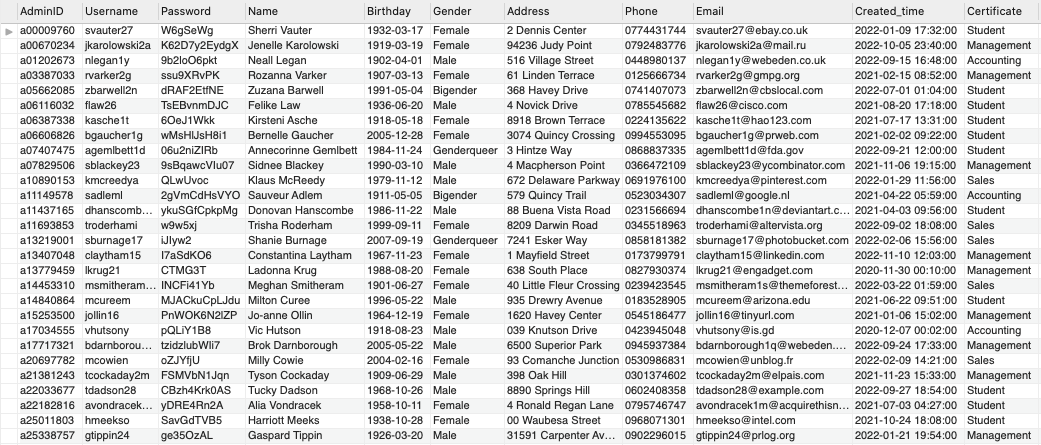
\includegraphics[width=\textwidth]{images/ADMIN.png}
    \caption{Bảng Admin}
\end{figure}

\begin{figure}[H]
    \centering
    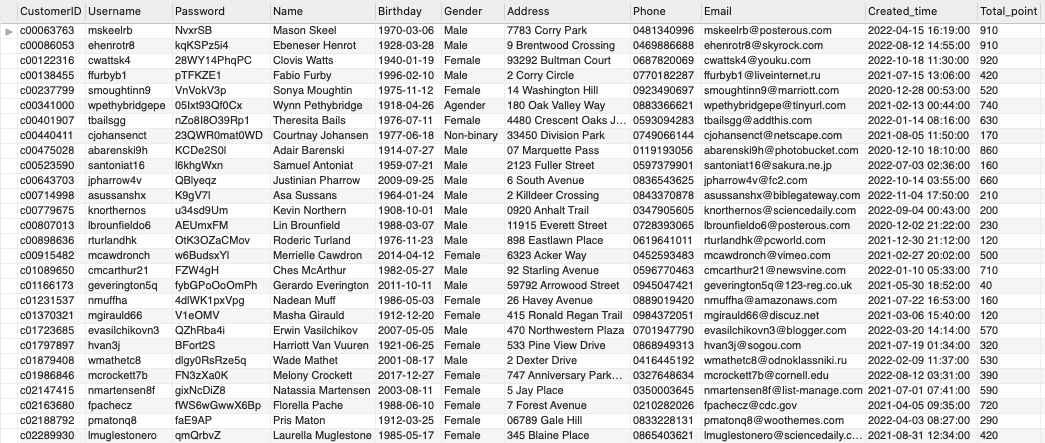
\includegraphics[width=\textwidth]{images/CUSTOMER.png}
    \caption{Bảng Customer}
\end{figure}

\begin{figure}[H]
    \centering
    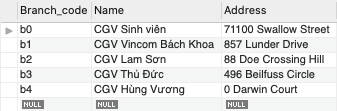
\includegraphics[width=10cm]{images/THATRE.png}
    \caption{Bảng Theatre}
\end{figure}

\begin{figure}[H]
    \centering
    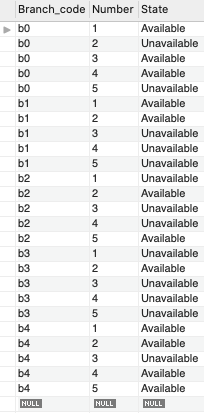
\includegraphics[width=5cm]{images/ROOM.png}
    \caption{Bảng Room}
\end{figure}

\begin{figure}[H]
    \centering
    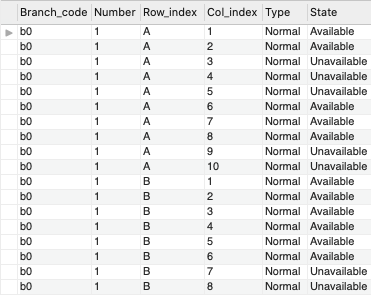
\includegraphics[width=10cm]{images/SEAT.png}
    \caption{Bảng Seat}
\end{figure}

\begin{figure}[H]
    \centering
    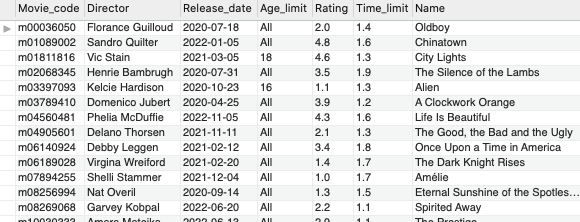
\includegraphics[width=\textwidth]{images/MOVIE.png}
    \caption{Bảng Movie}
\end{figure}

\begin{figure}[H]
    \centering
    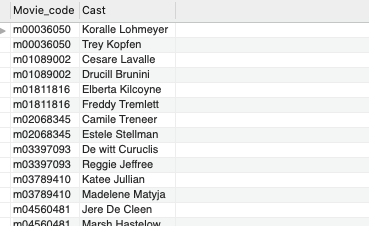
\includegraphics[width=10cm]{images/CAST.png}
    \caption{Bảng Movie\_cast}
\end{figure}

\begin{figure}[H]
\begin{subfigure}{.5\textwidth}
  \centering
  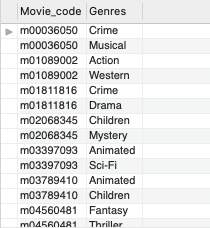
\includegraphics[width=.8\linewidth]{images/GENRES.png}
\end{subfigure}%
\begin{subfigure}{.5\textwidth}
  \centering
  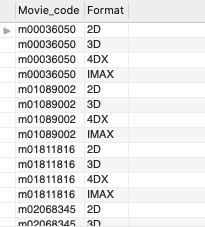
\includegraphics[width=.8\linewidth]{images/FORMAT.png}
\end{subfigure}
\caption{Bảng Movie\_genres và Movie\_format}
\end{figure}

\begin{figure}[H]
\begin{subfigure}{.5\textwidth}
  \centering
  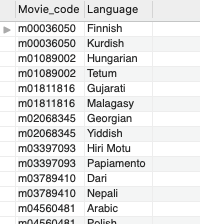
\includegraphics[width=.8\linewidth]{images/LANGUAGE.png}
\end{subfigure}%
\begin{subfigure}{.5\textwidth}
  \centering
  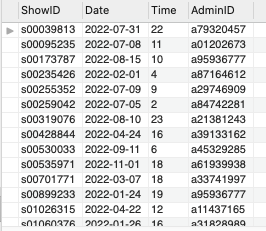
\includegraphics[width=.8\linewidth]{images/MOVIE_SHOW.png}
\end{subfigure}
\caption{Bảng Movie\_language và Movie\_show}
\end{figure}

\begin{figure}[H]
    \centering
    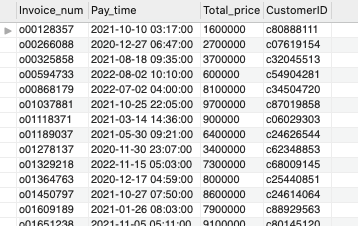
\includegraphics[width=12cm]{images/ORDER.png}
    \caption{Bảng cOrder}
\end{figure}

\begin{figure}[H]
\begin{subfigure}{.5\textwidth}
  \centering
  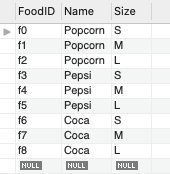
\includegraphics[width=.8\linewidth]{images/FOOD.png}
\end{subfigure}%
\begin{subfigure}{.5\textwidth}
  \centering
  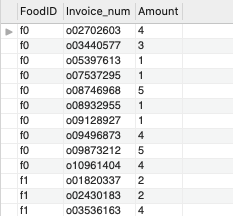
\includegraphics[width=.8\linewidth]{images/FOOD_ORDER.png}
\end{subfigure}
\caption{Bảng Food và Food\_order}
\end{figure}

\begin{figure}[H]
    \centering
    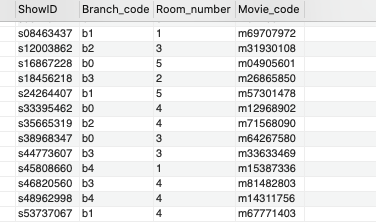
\includegraphics[width=12cm]{images/SCHEDULED.png}
    \caption{Bảng Scheduled}
\end{figure}

\begin{figure}[H]
    \centering
    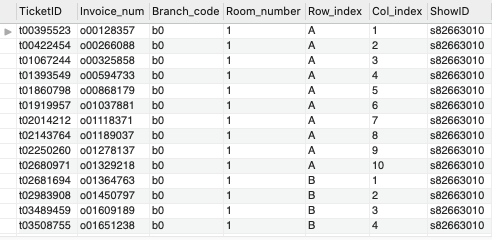
\includegraphics[width=12cm]{images/TICKET.png}
    \caption{Bảng Ticket}
\end{figure}

\begin{figure}[H]
    \centering
    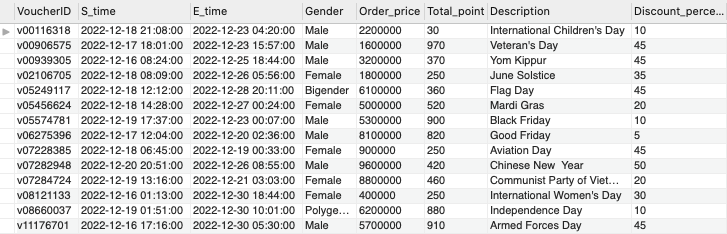
\includegraphics[width=15cm]{images/VOUCHER.png}
    \caption{Bảng Voucher}
\end{figure}

\begin{figure}[H]
    \centering
    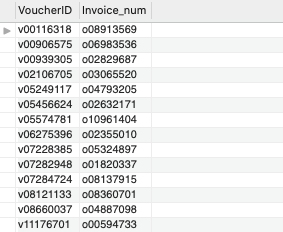
\includegraphics[width=10cm]{images/IS_APPLIED.png}
    \caption{Bảng isApplied}
\end{figure}


\section{Trigger - Thủ tục - Hàm}
\subsection{Thủ tục INSERT/UPDATE/DELETE dữ liệu trong một bảng dữ liệu}
Bảng dữ liệu: \textbf{CUSTOMER}
    \subsubsection{Thủ tục INSERT}
    Mô tả thủ tục: Dùng để thêm một tài khoản Customer trong bảng Customer. \\
    Câu lệnh tạo thủ tục:
    \begin{minted}{mysql}
        DROP PROCEDURE IF EXISTS insert_new_customer;
        DELIMITER //
        CREATE PROCEDURE insert_new_customer (
	IN
        CustomerID      VARCHAR(255),
	Username        VARCHAR(255),
	Password        VARCHAR(255),
	Name            VARCHAR(255),
	Birthday        DATE,
	Gender          VARCHAR(255),
	Address         VARCHAR(255),
	Phone           VARCHAR(255),
	Email           VARCHAR(255),
	Created_time    DATETIME,
	Total_point     BIGINT
	)
	BEGIN
    	DECLARE canAdd BOOL DEFAULT 1;
            -- Check customerID 
            IF length(CustomerID) < 9 THEN
                SELECT 'The customer ID is too short!'AS response_customer;
            SET canAdd = 0;
            ELSEIF length(CustomerID) > 9 THEN
                SELECT 'The customer ID is too long!' AS response_customer;
            SET canAdd = 0;
            ELSEIF CustomerID NOT REGEXP '^c[0-9]{8}' THEN
                SELECT 'The customer ID is invalid!' AS response_customer;
            SET canAdd = 0;
            END IF;
            -- Check username already exists
            IF EXISTS(SELECT * FROM customer where customer.Username=Username) THEN
                SELECT "The Username already exists"  AS response_customer;
                SET canAdd = 0;
            END IF;
            -- Check length of password
            IF length(Password) <= 5 THEN
                SELECT 'The length of password must be more than 5' AS response_customer;
            SET canAdd = 0;
            END IF;
            -- Check birthday
            IF (SELECT CONVERT(Birthday, DATE)) > (SELECT CURRENT_DATE) THEN
                SELECT "The Birthday is not correct!" AS response_customer;
                SET canAdd = 0;
            END IF;

            -- Check gender
            IF ((Gender != 'Male') and (Gender != 'Female') and (Gender != 'Other')) THEN
                SELECT "Gender is not correct!" AS response_customer;
                SET canAdd = 0;
            END IF;
            -- Check phone number
            IF (length(Phone) != 10) or (Phone NOT REGEXP "[0-9]{10}") THEN
                SELECT "Phone is not correct!" AS response_customer;
                SET canAdd = 0;
            END IF;
            -- Check Created_time
            IF (SELECT CONVERT(Created_time, DATE)) > (SELECT CURRENT_DATE) THEN
        	SELECT "Time is created more than present" AS response_customer;
            SET canAdd = 0;
            END IF;
            -- Check total point
            IF (Total_point < 0) THEN
                SELECT "Total point of customer must be greater than or equal to 0" AS reponse_customer;
            SET canAdd = 0;
            END IF;
        IF canAdd = 1 THEN
        INSERT INTO cinema.customer(CustomerID, Username, Password, Name, Birthday, Gender, Address, Phone, Email, Created_time, Total_point) 
        VALUES (customerID, Username, Password, Name, Birthday, Gender, Address, Phone, Email, Created_time , Total_point);
        SELECT "Insert Successful" as response_customer;
        END IF;
    END //
DELIMITER ;
    \end{minted}
    Câu lệnh thực thi thủ tục INSERT:
    \begin{minted}{mysql}
    call insert_new_customer('c12122022', 'bkuhcmut', '202220022Bk.', 'Bach Khoa', '1957-10-27', 'Other', '268 Ly Thuong Kiet', '0987654321', 'bku@hcmut.vn', '2022-08-06 2:20', 580);
    \end{minted}
    
    Kết quả màn hình hiển thị từ DBMS: 

    \begin{figure}[h]
        \centering
        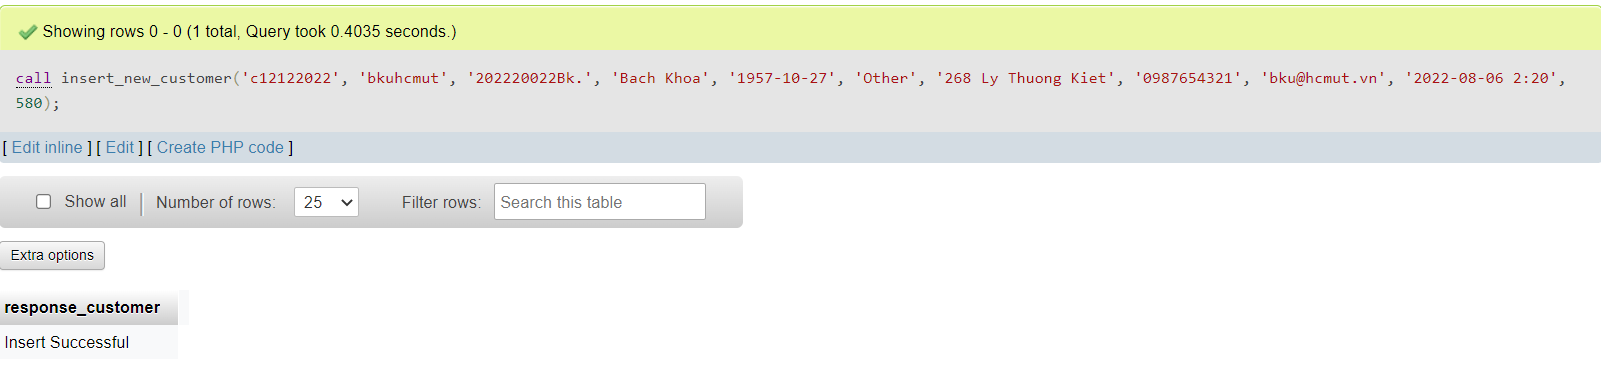
\includegraphics[scale=0.5]{images/insertNewCustomer.png}
    \end{figure}
    
    \subsubsection{Thủ tục UPDATE}
    Nội dung thủ tục: Cập nhật thông tin một tài khoản Customer trong bảng Customer. Các mục thông tin có thể được cập nhật bao gồm Mật khẩu, Địa chỉ, Số điện thoại, Email, Tên, Giới tính, Sinh nhật của khách hàng. 
    \begin{minted}{mysql}
        DROP PROCEDURE IF EXISTS update_password_customer;
        DELIMITER //
        CREATE PROCEDURE update_password_customer (
	IN
        CID     VARCHAR(255),
	Pass    VARCHAR(255)
	)
	BEGIN
        IF length(Pass) <= 5 THEN
			SELECT 'The length of password must be more than 5' AS response;
        ELSEIF NOT EXISTS (SELECT * from customer where customer.CustomerID=CID) THEN
            SELECT "Customer doesn't exist!" AS response;
        ELSE
        	UPDATE customer SET customer.Password = Pass WHERE customer.CustomerID = CID;
        END IF;
        END //
        DELIMITER ;

        DROP PROCEDURE IF EXISTS update_address_customer;
        DELIMITER //
        CREATE PROCEDURE update_address_customer (
	IN
        usrName		VARCHAR(255),
	Addr 		VARCHAR(255)
	)
	BEGIN
    	IF EXISTS (SELECT * from customer where customer.Username = usrName) THEN
            UPDATE customer SET customer.Address=Addr where customer.Username = usrName;
            SELECT "Update Address Successful";
        ELSE
            SELECT "Customer doesn't exist!" as response;
            END IF;
        END //
        DELIMITER ;
        DROP PROCEDURE IF EXISTS update_phone_customer;
        
        DELIMITER //
        CREATE PROCEDURE update_phone_customer (
	IN
        usrName		VARCHAR(255),
	phoneNumber 		VARCHAR(255)
	)
	BEGIN
        IF (length(phoneNumber) != 10) or (phoneNumber NOT REGEXP "^0[0-9]{9}") THEN
			SELECT "Phone is not correct!" AS response;
        ELSEIF NOT EXISTS (SELECT * from customer where customer.Username = usrName) THEN
            SELECT "Customer doesn't exist!" AS response;
        ELSE
        	UPDATE customer SET customer.Phone = phoneNumber where customer.Username = usrName;
        	SELECT "Update Phone Number Is Successful" AS response;
        END IF;
        END //
        DELIMITER ;

        DROP PROCEDURE IF EXISTS update_email_customer;
        DELIMITER //
        CREATE PROCEDURE update_email_customer (
        IN
        usrName   VARCHAR(255),
        mail      VARCHAR(255)
        )
        BEGIN
        IF NOT EXISTS (SELECT * from customer where customer.Username = usrName) THEN
            SELECT "Customer doesn't exists!" AS response;
        ELSEIF (mail NOT REGEXP "^[A-Za-z]+[A-Za-z0-9.]+@[A-Za-z0-9.-]+\.[A-Za-z]{2,4}$") THEN
            SELECT "Email is not correct!" AS response;
        ELSE
        	UPDATE customer SET customer.Email = mail where customer.Username = usrName;
        	SELECT "Update Email Successfull" as response;
        END IF;
        END //
        DELIMITER ;

        DROP PROCEDURE IF EXISTS update_name_customer;
        DELIMITER //
        CREATE PROCEDURE update_name_customer (
        IN
        usrName       VARCHAR(255),
        fullName      VARCHAR(255)
        )
        BEGIN
        IF NOT EXISTS (SELECT * from customer where customer.Username = usrName) THEN
            SELECT "Customer doesn't exists!" AS response;
        ELSE
        	UPDATE customer SET customer.Name = fullName where customer.Username = usrName;
        	SELECT "Update Name Successfull" as response;
        END IF;
        END //
        DELIMITER ;

        DROP PROCEDURE IF EXISTS update_gender_customer;
        DELIMITER //
        CREATE PROCEDURE update_gender_customer (
        IN
        usrName VARCHAR(255),
        sex      VARCHAR(255)
        )
        BEGIN
        IF NOT EXISTS (SELECT * from customer where customer.Username = usrName) THEN
            SELECT "Customer doesn't exists!" AS response;
        ELSEIF ((sex != 'Male') and (sex != 'Female') and (sex != 'Other')) THEN
			SELECT "Gender is not correct!" AS response;
		ELSE
        	UPDATE customer SET customer.Gender = sex where customer.Username = usrName;
        	SELECT "Update Gender Successfull" as response;
        END IF;
        END //
        DELIMITER ;


        DROP PROCEDURE IF EXISTS update_birthday_customer;
        DELIMITER //
        CREATE PROCEDURE update_birthday_customer (
        IN
        usrName VARCHAR(255),
        bornDay      DATE
        )
        BEGIN
        IF NOT EXISTS (SELECT * from customer where customer.Username = usrName) THEN
            SELECT "Customer doesn't exists!" AS response;
        ELSEIF (SELECT CONVERT(bornDay, DATE)) > (SELECT CURRENT_DATE) THEN
        	SELECT "The Birthday is not correct!" AS response;
		ELSE
        	UPDATE customer SET customer.Birthday = bornDay where customer.Username = usrName;
        	SELECT "Update Birthday Successfull" as response;
        END IF;
        END //
        DELIMITER ;
    \end{minted}
    Câu lệnh thực thi thủ tục UPDATE:
    \begin{minted}{mysql}
    call update_birthday_customer('bkuhcmut', '1967-10-27')
    \end{minted}
     Kết quả màn hình hiển thị từ DBMS: 
    \begin{figure}[h]
        \centering
        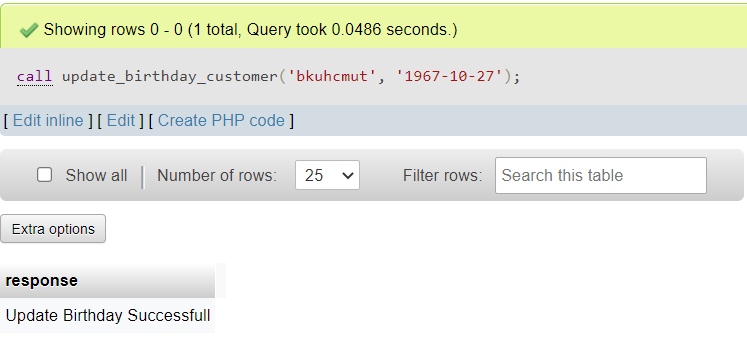
\includegraphics[scale=0.5]{images/updateBirthday.png}
    \end{figure}
    \subsubsection{Thủ tục DELETE}
    Nội dung thủ tục: Xoá môt tài khoản Customer trong bảng Customer.      
    \begin{minted}{mysql}
    DROP PROCEDURE IF EXISTS delete_customer;
    DELIMITER //
    CREATE PROCEDURE delete_customer (
    IN
        CustomerID		VARCHAR(255)
    )
    BEGIN
        IF length(CustomerID) < 9 THEN
        SELECT 'The customer ID is too short!'AS response;
        ELSEIF length(CustomerID) > 9 THEN
        SELECT 'The customer ID is too long!' AS response;
        ELSEIF CustomerID NOT REGEXP '^c[0-9]{8}' THEN
        SELECT 'The customer ID is invalid!' AS response;
        ELSE
            DELETE FROM customer WHERE customer.customerID=customerID;
            SELECT 'Customer Deleted Successfully!' AS response;
        END IF;
    END //
    DELIMITER ;
  \end{minted}
Câu lệnh thực thi thủ tục DELETE:
\begin{minted}{mysql}
    call delete_customer('c12122022')
\end{minted}
Kết quả màn hình hiện thị từ DBMS:

\begin{figure}[h]
    \centering
    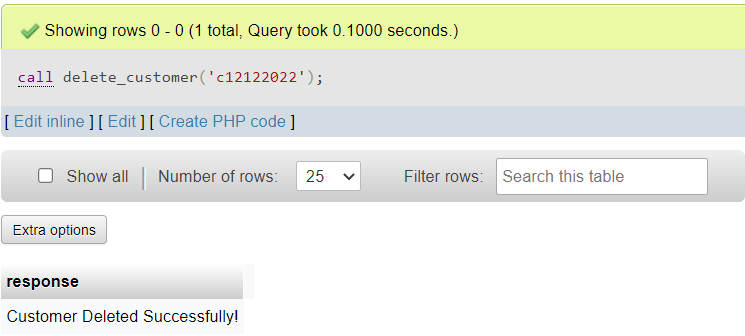
\includegraphics{images/deleteCustomer.png}
\end{figure}
   
    
\subsection{Trigger}
     \subsubsection{Trigger 1}
\textbf{Nội dung Trigger:} Mỗi khi khách hàng (Customer) thanh toán một đơn hàng, khách hàng đó sẽ nhận được một lượng điểm tích luỹ có giá trị bằng với tổng tiền đơn hàng chia 1000.
\begin{itemize}
    \item[--] Điều kiện kích hoạt Trigger: Một đơn hàng được thêm vào bảng \textbf{cOrder}.
    \item[--] Thao tác được thực hiện khi Trigger được kích hoạt: sau khi sự kiện kích hoạt, giá trị \textbf{Total\_point} của bảng \textbf{Customer} được cập nhật (cộng thêm 1 lượng $Total_price/1000$).
\end{itemize}
\textbf{Lệnh tạo Trigger:}
\begin{minted}{mysql}
    DROP TRIGGER IF EXISTS addTotalPoint;
    CREATE TRIGGER addTotalPoint
        AFTER INSERT ON cOrder
        FOR EACH ROW
	   UPDATE Customer
	   SET Total_point = Total_point + NEW.Total_price/1000
	   WHERE CustomerID = NEW.CustomerID;
\end{minted}
Câu lệnh thực thi trigger 1:
\begin{minted}{mysql}
    INSERT INTO cOrder (Invoice_num, Pay_time, Total_price, CustomerID)
    VALUES ('o11111111', '2022-11-02 19:07:34', 230000, 'c12345678');
\end{minted}
Kết quả màn hình hiển thị từ DBMS:
Trước khi gọi insert cOrder:
\begin{figure}[h]
    \centering
    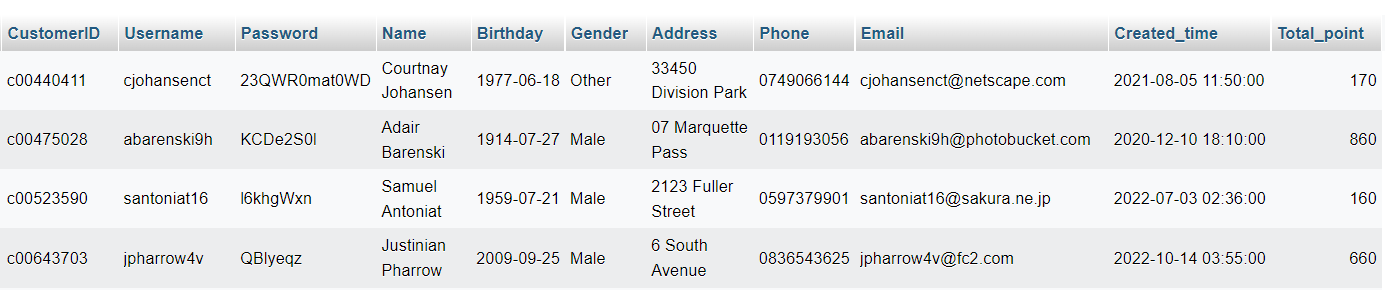
\includegraphics[scale=0.5]{images/addTotalPoint1.png}
\end{figure}

Sau khi gọi insert cOrder:
\begin{figure}[h]
    \centering
    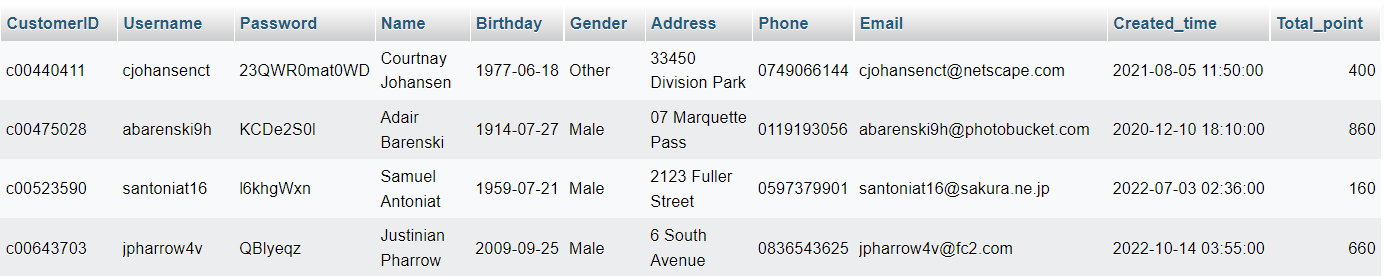
\includegraphics[scale=0.5]{images/addTotalPoint2.png}
\end{figure}
    \subsubsection{Trigger 2}
Nội dung Trigger: Nếu một voucher có điều kiện sử dụng là dùng 1 lượng Total\_point thì khách hàng sử dụng Voucher đó sẽ bị trừ một lượng Total\_point tương ứng đã tích luỹ.
\begin{itemize}
    \item[--] Điều kiện kích hoạt Trigger: ngay sau khi 1 giá trị Voucher đã được dùng. Tức một hàng mới được thêm vào bảng \textbf{isApplied}.
    \item[--] Thao tác được thực hiện khi Trigger được kích hoạt: Lấy ra điểm tích luỹ được yêu cầu trong Voucher và trừ một lương tương ứng vào điểm tích luỹ (\textbf{Total\_point}) của người dùng.
\end{itemize}

\begin{minted}{mysql}
    DROP TRIGGER IF EXISTS useTotalPoint;
    DELIMITER //
    CREATE TRIGGER useTotalPoint
    AFTER INSERT ON isApplied
    FOR EACH ROW
        BEGIN
            SET @point = (
                SELECT Total_point 
                FROM Voucher
                WHERE VoucherID = NEW.VoucherID
            );
            IF @point IS NOT NULL THEN
                SET @cID = (
                    SELECT CustomerID
                    FROM cOrder
                    WHERE Invoice_num = NEW.Invoice_num
                    );
                    UPDATE Customer
                    SET Total_point = Total_point - @point
                    WHERE CustomerID = @cID;
                    END IF;
        END //
    DELIMITER ;
\end{minted}   

Câu lệnh thực thi trigger 2:
Giả sử đã có voucher với VoucherID = "v22222222" và một order của khách hàng với Invoice\_num="o33333333" trong database:
\begin{minted}{mysql}
    INSERT INTO isApplied(VoucherID, Invoice_num) VALUES('v22222222','o33333333');
\end{minted}
Kết quả màn hình hiển thị từ DBMS:

Trước khi thực thi lệnh insert ở trên:
\begin{figure}[h]
    \centering
    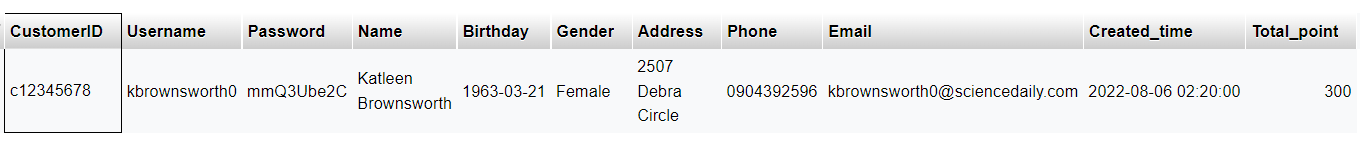
\includegraphics[scale=0.5]{images/useTotalPoint1.png}
\end{figure}
\newpage
Sau khi thực thi lệnh insert ở trên:
\begin{figure}[h]
    \centering
    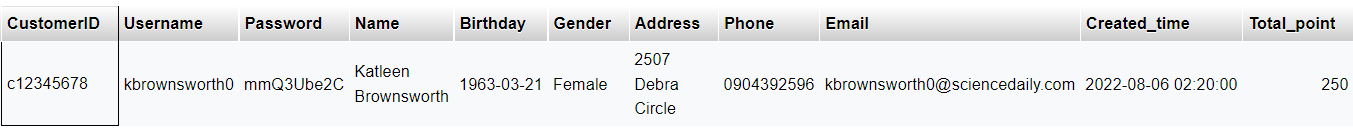
\includegraphics[scale=0.5]{images/useTotalPoint2.png}
\end{figure}

\subsection{Thủ tục}
\subsubsection{Thủ tục 1}
Nội dung thủ tục 1: Xuất ra thông tin tất cả khách hàng theo giới tính (Male, Female, Other) và có ít nhất một hóa đơn có tổng số tiền (\textbf{Total\_price}) lớn hơn hoặc bằng yêu cầu đặt ra.

Các bảng sử dụng: Customer, cOrder.
\begin{minted}{mysql}
    DROP PROCEDURE IF EXISTS customer_orders;
    DELIMITER //
    CREATE PROCEDURE customer_orders (
        IN
        Gender VARCHAR(50),
        minPrice FLOAT
    )
    BEGIN
        IF (Gender = 'Male' or Gender = 'Female' or Gender = 'Other') THEN
            SELECT Customer.Username,Customer.Password,Customer.Email, Customer.Name, Customer.Birthday, Customer.Address, Customer.Phone, Customer.Gender,Customer.Total_point, cOrder.Total_price FROM Customer, cOrder
            WHERE Customer.CustomerID = cOrder.CustomerID AND Customer.Gender = Gender AND cOrder.Total_price >= minPrice
            ORDER BY Customer.Name;
        END IF;
    END //
    DELIMITER ;
\end{minted}
Câu lệnh thực thi thủ tục 1:
\begin{minted}{mysql}
   call customer_orders('Male', 98000000);
\end{minted}
\newpage
Kết quả màn hình hiển thị từ DBMS:
\begin{figure}[h]
    \centering
    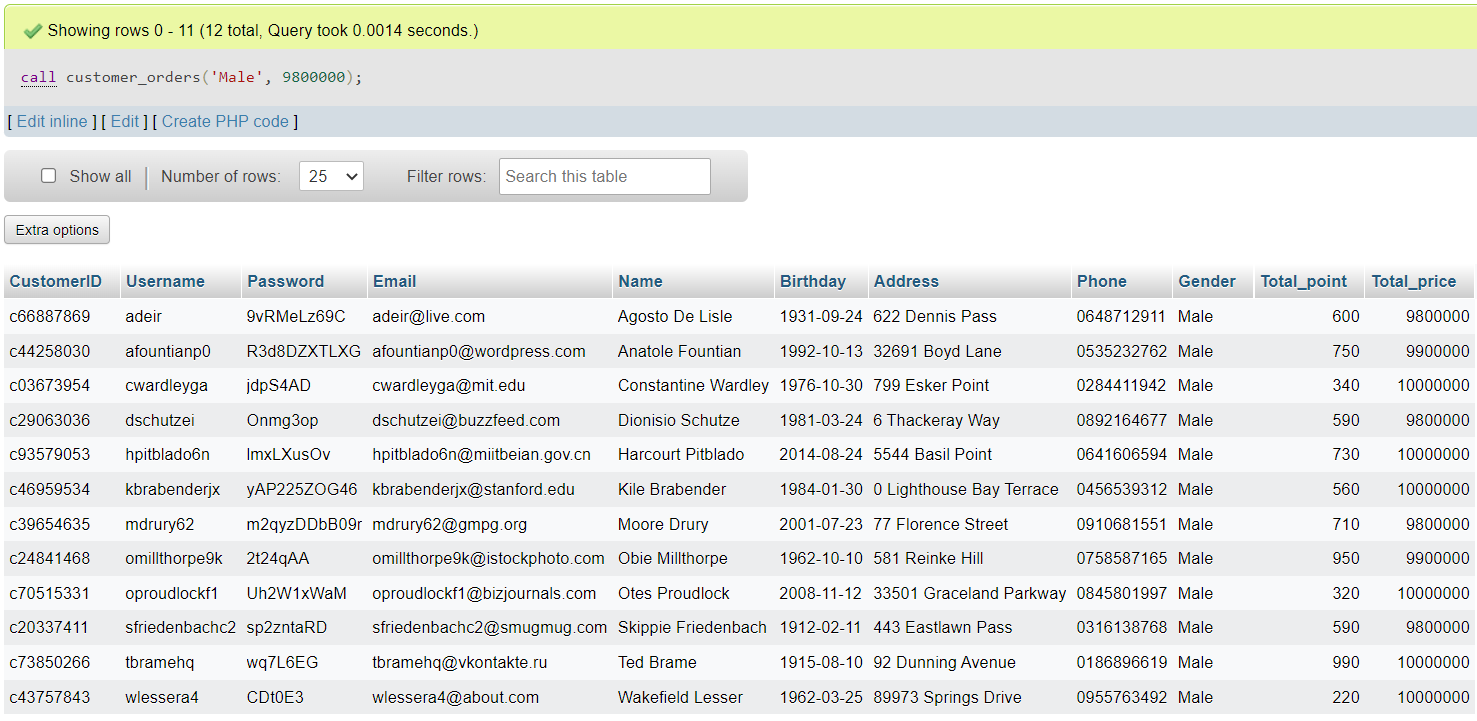
\includegraphics[scale=0.5]{images/customercOrder.png}
\end{figure}
\subsubsection{Thủ tục 2}
Nội dung thủ tục 2: Xuất ra thông tin những khách hàng đã đặt hàng từ một ngày nhất định đến hiện tại mà theo tên thức ăn và có số lượng lớn hơn số lượng để ra.  
% anh ơiiii hihi

Các bảng sử dụng: Food, cOrder, Food\_order, Customer.
\begin{minted}{mysql}
    DROP PROCEDURE IF EXISTS findOrderAfter;
    DELIMITER //
    CREATE PROCEDURE findOrderAfter(
     IN
        DateFrom DATE,
        Amount INT, 
        NameFood VARCHAR(255),
        sortPatemeter VARCHAR(255),
        offset INT
    )
    BEGIN
        IF NOT EXISTS(SELECT * FROM Food WHERE Name=NameFood) THEN
            SELECT "The food name doesn't exist!" AS Response;
        ELSEIF (sortPatemeter= 'Name') THEN
            SELECT  Customer.Username, Customer.Gender, Customer.Name, Customer.Birthday,       Customer.Address, Customer.Phone, SUM(Food_order.Amount) AS OrderAmount
            FROM Food, cOrder, Food_order, Customer
            WHERE CONVERT(cOrder.Pay_time, DATE) > DateFrom
                AND Food_order.Invoice_num=cOrder.Invoice_num
                AND Food.FoodID=Food_order.FoodID
                AND cOrder.CustomerID=Customer.CustomerID
                AND Food.Name=NameFood
            GROUP BY Customer.Name
            HAVING  SUM(Food_order.Amount) > Amount
            ORDER BY Customer.Name
            LIMIT 10 OFFSET offset;

        ELSEIF (sortPatemeter = 'Amount') THEN
            SELECT  Customer.Username, Customer.Gender, Customer.Name, Customer.Birthday, Customer.Address, Customer.Phone, SUM(Food_order.Amount) AS OrderAmount
            FROM Food, cOrder, Food_order, Customer
            WHERE CONVERT(cOrder.Pay_time, DATE) > DateFrom
                AND Food_order.Invoice_num=cOrder.Invoice_num
                AND Food.FoodID=Food_order.FoodID
                AND cOrder.CustomerID=Customer.CustomerID
                AND Food.Name=NameFood
            GROUP BY Customer.Name
            HAVING  SUM(Food_order.Amount) > Amount
            ORDER BY SUM(Food_order.Amount)
            LIMIT 10 OFFSET offset;

        ELSE
            SELECT  Customer.Username, Customer.Gender, Customer.Name, Customer.Birthday, Customer.Address, Customer.Phone, SUM(Food_order.Amount) AS OrderAmount
            FROM Food, cOrder, Food_order, Customer
            WHERE CONVERT(cOrder.Pay_time, DATE) > DateFrom
                AND Food_order.Invoice_num=cOrder.Invoice_num
                AND Food.FoodID=Food_order.FoodID
                AND cOrder.CustomerID=Customer.CustomerID
                AND Food.Name=NameFood
            GROUP BY Customer.Username
            HAVING  SUM(Food_order.Amount) > Amount
            ORDER BY Customer.Username
            LIMIT 10 OFFSET offset;

        END IF;
    END //
    DELIMITER ;
\end{minted}
Câu lệnh thực thi thủ tục 2:
\begin{minted}{mysql}
    call findOrderAfter('2022-01-01', 2, 'Coca');
\end{minted}
\newpage
Kết quả màn hình hiển thị từ DBMS:
\begin{figure}[h]
    \centering
    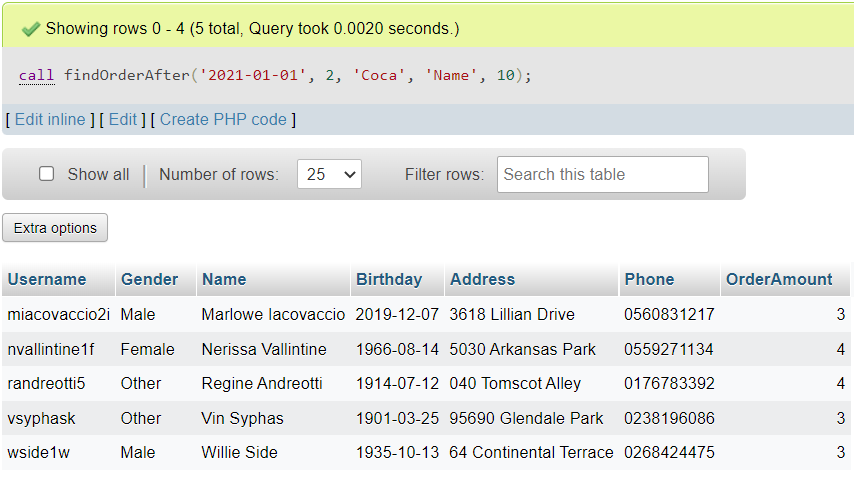
\includegraphics[scale=0.7]{images/findOrderAfter.png}
\end{figure}
\subsection{Hàm}
\subsubsection{Hàm 1}
Nội dung Hàm 1: Hàm tính xem đến ngày thứ bao nhiêu trong tháng thì rạp phim X đạt chỉ tiêu doanh thu đặt ra của tháng Y.
Các bảng sử dụng: Theatre, Ticket.
\begin{itemize}
    \item[--] Tham số đầu vào: Tháng, năm, rạp và chỉ tiêu đặt ra.
    
    \item[--] Tham số đầu ra: Ngày đạt được chỉ tiêu, tháng đó có đạt chỉ tiêu đề ra hay không.
   
\end{itemize}

\begin{minted}{mysql}
    DROP FUNCTION IF EXISTS dayReachTarget;
    DELIMITER //
    CREATE FUNCTION dayReachTarget(
        month   INT,
        year    INT,
        bCode   VARCHAR(255),
        target  INT)
    RETURNS     VARCHAR(255)
    BEGIN
        DECLARE rev INT DEFAULT 0;
        DECLARE d VARCHAR(2) DEFAULT '';
        -- CHECK INPUT
        IF (month < 0 OR month > 12) THEN
            RETURN 'THE VALUE OF MONTH MUST BE FROM 1 - 12';
        END IF;
        IF (year < 1999 OR year > YEAR(CURDATE())) THEN
            RETURN CONCAT('THE VALUE OF YEAR MUST BE FROM 1999 - ', YEAR(CURDATE()));
        END IF;
        IF (CHAR_LENGTH(bCode) <> 2 OR LEFT(bCode, 1) <> 'b') THEN
            RETURN 'INVALID VALUE OF BRANCH CODE';
        END IF;
        IF (target < 0 OR target > 500000000) THEN
            RETURN 'INVALID VALUE OF TARGET';
        END IF;
        -- LOOP
        BEGIN
            DECLARE notReach INT DEFAULT 0;
            DECLARE price INT DEFAULT 0;
            DECLARE ptime DATE;
            DECLARE p CURSOR FOR SELECT *
            FROM (
                SELECT Total_price, Pay_time
                FROM (
                    SELECT DISTINCT Invoice_num
                    FROM Ticket
                    WHERE Branch_code = bCode
                ) t INNER JOIN cOrder ON t.Invoice_num = cOrder.Invoice_num
                WHERE MONTH(Pay_time) = month AND YEAR(Pay_time) = year
                ORDER BY Pay_time ASC -- < in case the times were not ordered correctly >
            ) pt;
            -- declare NOT FOUND handler
            DECLARE CONTINUE HANDLER 
            FOR NOT FOUND SET notReach = 1;
            OPEN p;
            isReach: LOOP
                IF (rev >= target OR notReach = 1) THEN LEAVE isReach;
                END IF;
                FETCH p INTO price, ptime;
                SET rev = rev + price;
                SET d = DAY(ptime);
            END LOOP isReach;
            CLOSE p;
        END;
        IF (rev > target) THEN 
            RETURN CONCAT('DOANH THU THANG ', month, ' NAM ', year, ' DAT CHI TIEU TRONG VONG ', d, ' NGAY');
        ELSE 
            RETURN CONCAT('DOANH THU THANG ', month , ' NAM ', year, ' KHONG DAT CHI TIEU');
        END IF;
    END //
    DELIMITER ;
\end{minted} 

Câu lệnh thực thi hàm 1:
\begin{minted}{mysql}
    select dayReachTarget(1, 2021,'b0', 10000000);
\end{minted}
Kết quả màn hình hiển thị từ DBMS:
\begin{figure}[h]
    \centering
    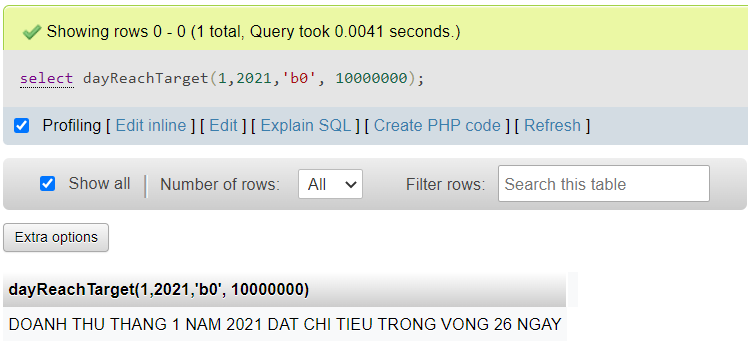
\includegraphics{images/dayReachTarget.png}
\end{figure}
 \subsubsection{Hàm 2}
Nội dung Hàm 2: Xét độ tuổi của khách hàng, có đạt điều kiện về mục giới hạn độ tuổi của phim mà họ muốn xem hay không.
Các bảng sử dụng: Customer, Movie.
\begin{itemize}
    \item[--] Tham số đầu vào: Mã khách hàng, mã phim.
    \item[--] Tham số đầu ra: Khách hàng đó có đủ tuổi để xem phim hay không.
\end{itemize}
\begin{minted}{mysql}
    DROP FUNCTION IF EXISTS checkAge;
    DELIMITER //
    CREATE FUNCTION checkAge(
        mCode   VARCHAR(255), 
        cID     VARCHAR(255))
    RETURNS VARCHAR(20)

    BEGIN
        DECLARE bday DATE;
        DECLARE age VARCHAR(3);
        -- CHECK INPUT
        IF (CHAR_LENGTH(mCode) <> 9 OR LEFT(mCode, 1) <> 'm') THEN
        RETURN 'INVALID VALUE OF MOVIE CODE';
        END IF;
    
        IF (CHAR_LENGTH(cID) <> 9 OR LEFT(cID, 1) <> 'c') THEN
        RETURN 'INVALID VALUE OF CUSTOMER ID';
        END IF;
    
        -- FUNCTION BODY
        SET bday = (SELECT Birthday
                    FROM Customer
                    WHERE CustomerID = cID);
        SET age = (SELECT Age_limit
                    FROM Movie
                    WHERE Movie_code = mCode);
        IF (YEAR(CURDATE()) - YEAR(bday)) >= age OR (age = 'All') THEN
            RETURN 'You are old enough';
        ELSE RETURN 'You are not old enough';
        END IF;
    END //
    DELIMITER ;
\end{minted}   
Câu lệnh thực thi hàm 2:
\begin{minted}{mysql}
    select checkAge('m78126847','c00440411');
\end{minted}

Kết quả màn hình hiển thị từ DBMS:
\begin{figure}[h]
    \centering
    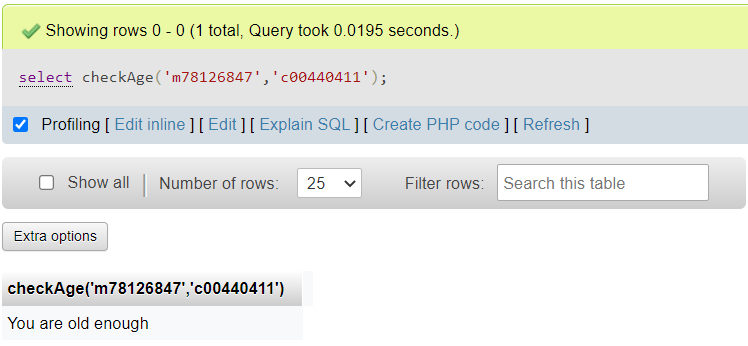
\includegraphics{images/checkAge.png}
\end{figure}
\section{Demo giao diện}
\subsection{Setup môi trường}
Đây là web được xây dựng từ HTML, CSS, JavaScript, PHP và MySQL. Ở đây có Xampp hỗ trợ môi trường để có thể chạy PHP và MySQL.

\begin{figure}[H]
    \centering
    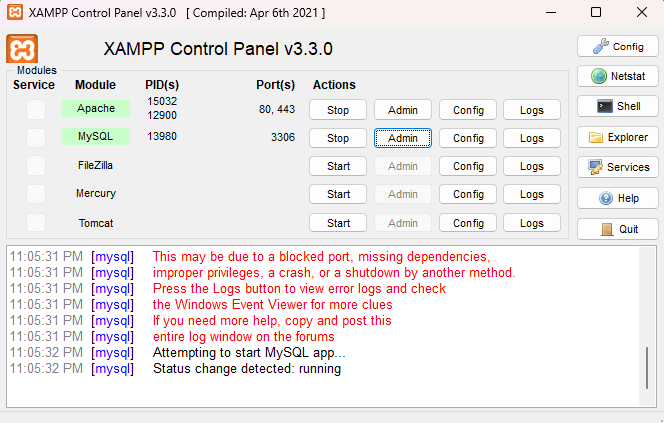
\includegraphics[scale=0.8]{images/xampp.png}
    \caption{Giao diện Xampp}
\end{figure}

Để chạy được PHP có liên kết với MySQL, đầu tiên chúng ta mở ứng dụng XAMPP. Sau đó chúng ta click vào tuần "Start" của Apache và MySQL. Có một lưu ý là nếu chúng ta có một ứng dụng khác chạy trên port "3306" của MySQL xampp đang chạy thì button "Start" sẽ chuyển thành "Stop".

\begin{figure}[H]
    \centering
    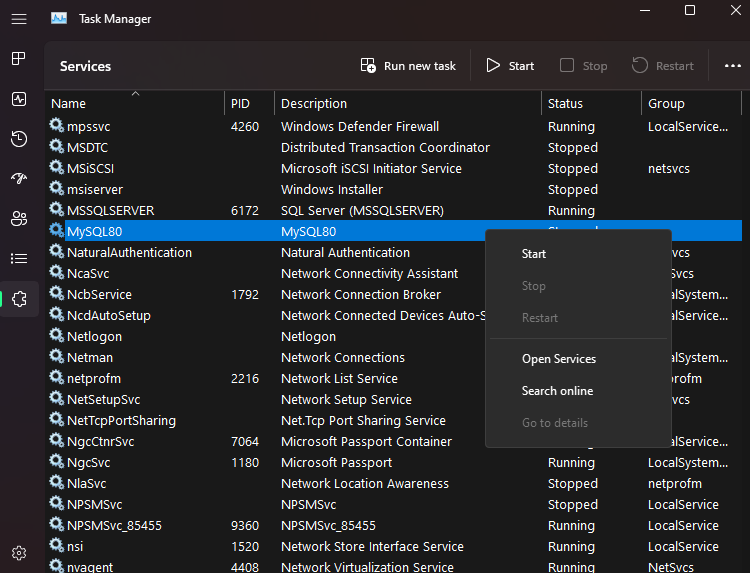
\includegraphics[scale=0.8]{images/taskManager.png}
    \caption{Task Manager}
\end{figure}

Chúng ta chọn vào Service và click chuột phải vào "MySQL80" và chọn "Stop".

\begin{figure}[H]
    \centering
    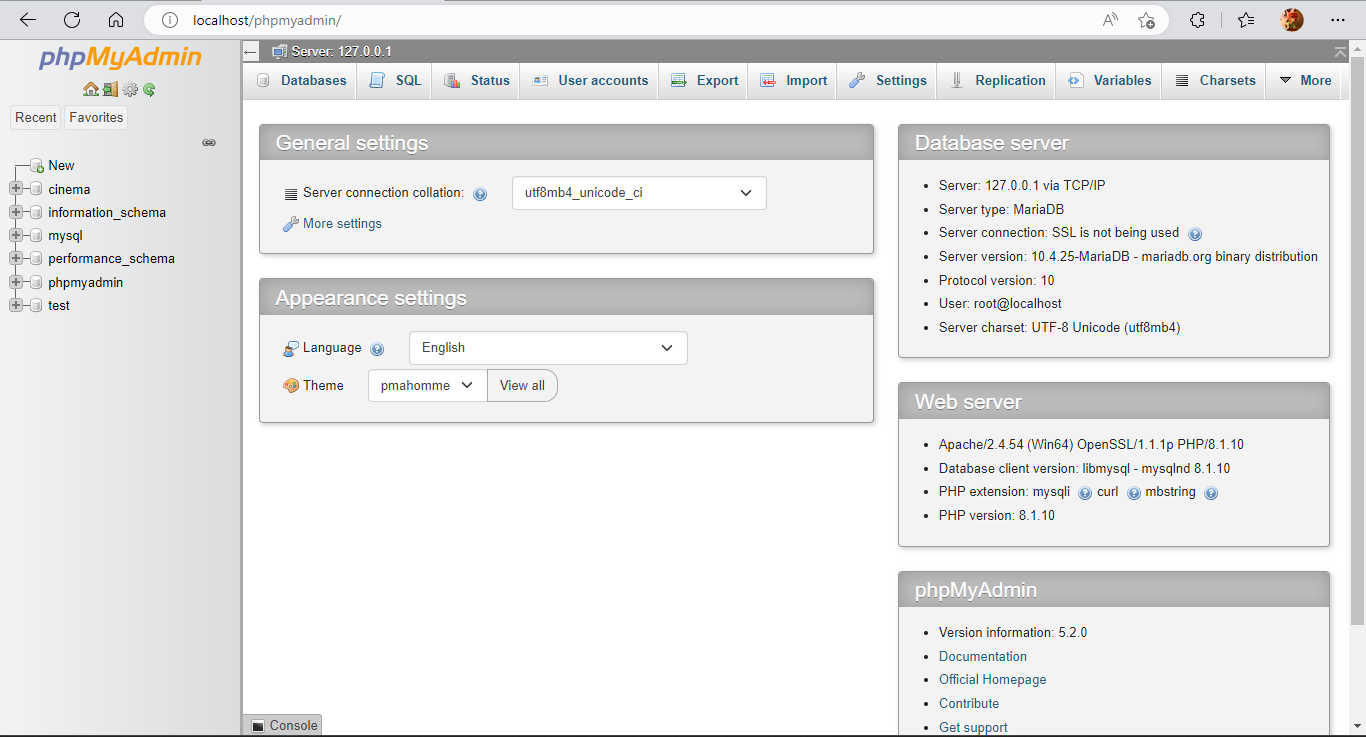
\includegraphics[scale=0.45]{images/phpAdmin.png}
    \caption{Giao diện phpMyAdmin}
\end{figure}
Sau khi MySQL trong XAMPP vẫn giữ trạng thái "Start" thì chúng ta đã khởi động thành công. Sau đó chúng ta click vào "Admin" sau "Start" của MySQL để chúng ta có thể vào giao diện phpMyAdmin.

\subsection{Các chức năng}
- Thêm, sửa và xóa các Customer.\\
- Tìm kiếm các Customer thỏa mãn một hoặc một số điều kiện được nhập vào.\\
- Tìm kiếm Order Food được thanh toán với một số lượng sau một ngày được nhập.\\
- Tìm kiếm ngày đạt được doanh thu được nhập vào trong tháng.\\
- Filter Customer theo giới tính, tổng số điểm tích lũy, theo số đơn hàng mua.\\
- Phân trang cho các sản phẩm có nhiều records.\\
- Sắp xếp theo thứ tự tăng dần hoặc giảm dần của các thuộc tính.\\

\subsection{Hiện thực}
\subsubsection{Home}
\begin{figure}[H]
    \centering
    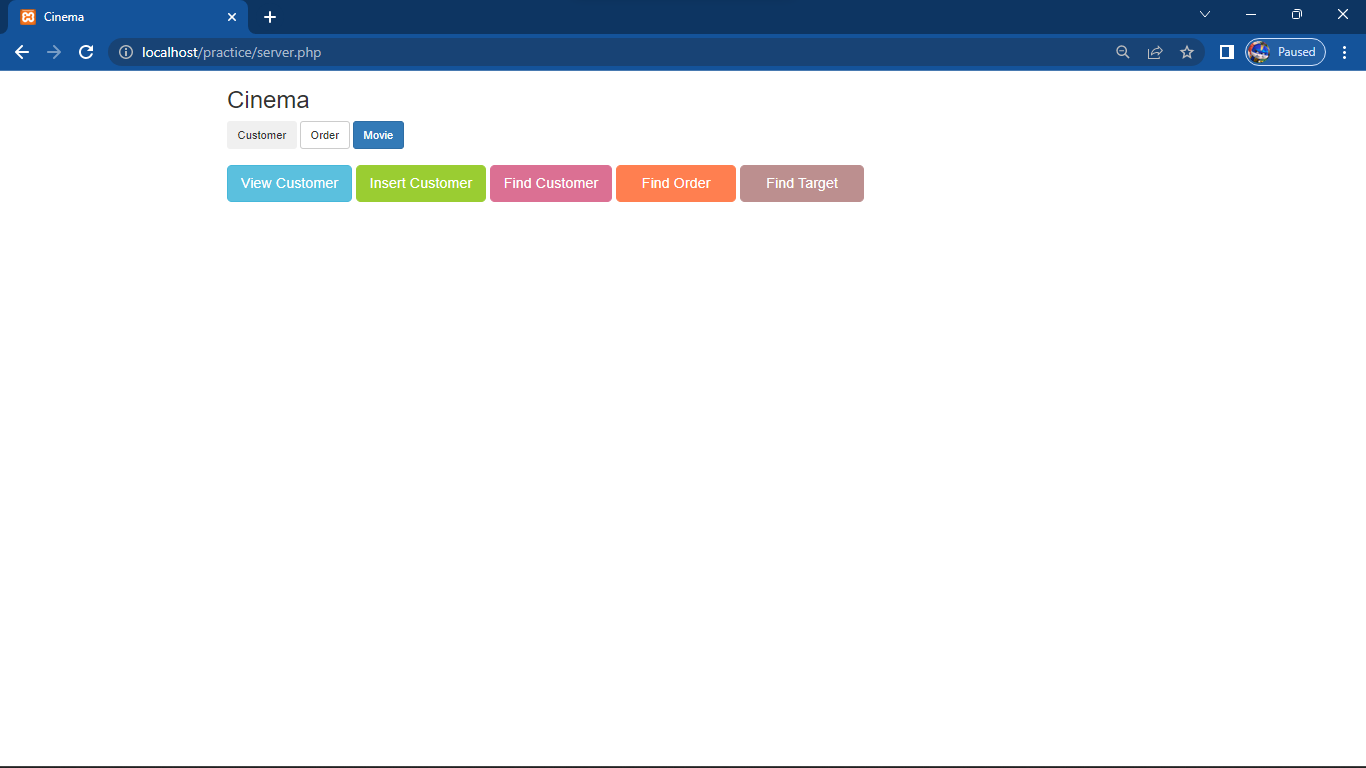
\includegraphics[scale=0.45]{images/viewCustomer.png}
    \caption{Home}
\end{figure}
Ở giao diện này có các đường liên kết điều hướng đến các giao diện khác.

\begin{figure}[H]
    \centering
    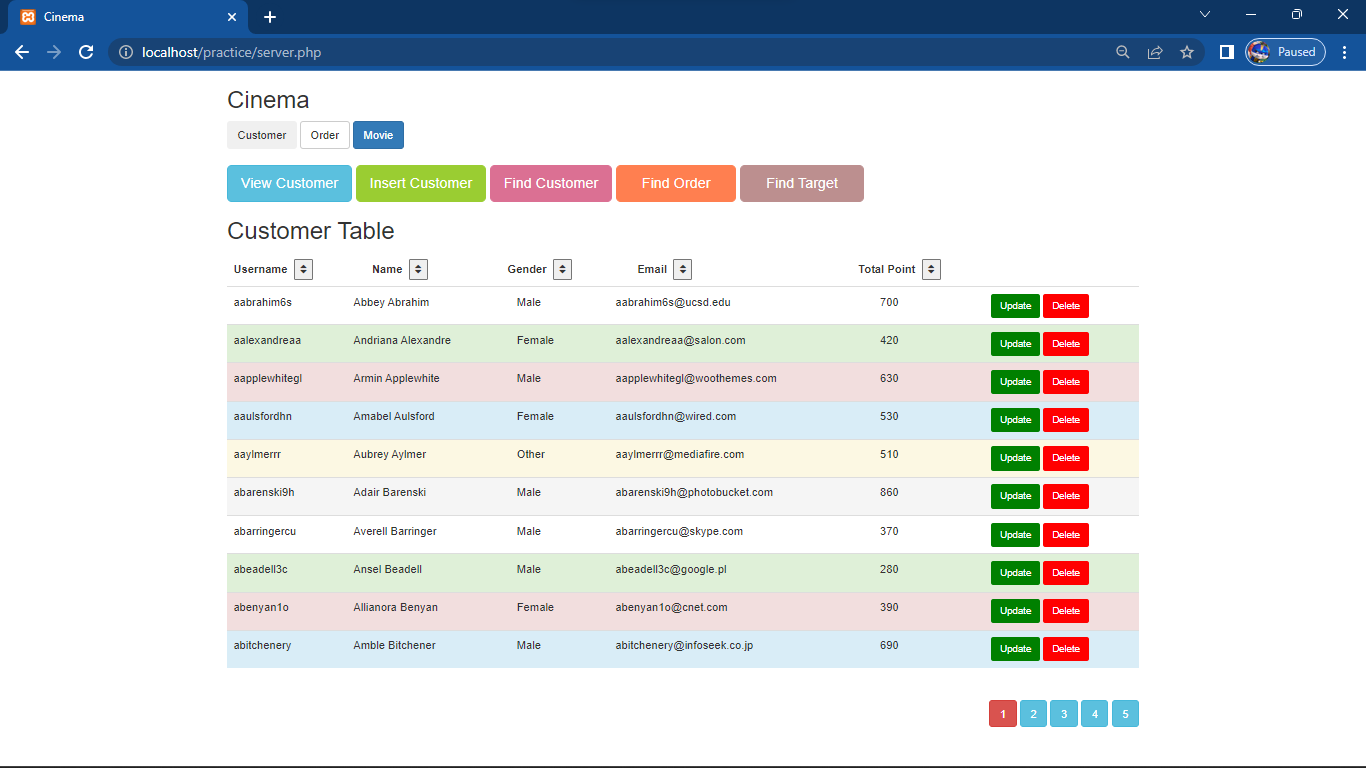
\includegraphics[scale=0.45]{images/viewAll.png}
    \caption{View Customer}
\end{figure}
Khi click vào "view Customer" thì sẽ hiển thị ra giao diện chứa những thông tin về Customer. Trong giao diện này, chúng ta có thể thực hiện các thao tác thêm, sửa và xóa các thông tin liên quan đến Customer. Ở mỗi thuộc tính được hiển thị, chúng ta có thể lựa chọn sắp xếp chúng theo thứ tự tăng hoặc giảm dần.


\subsubsection{Insert Customer}
\begin{figure}[H]
    \centering
    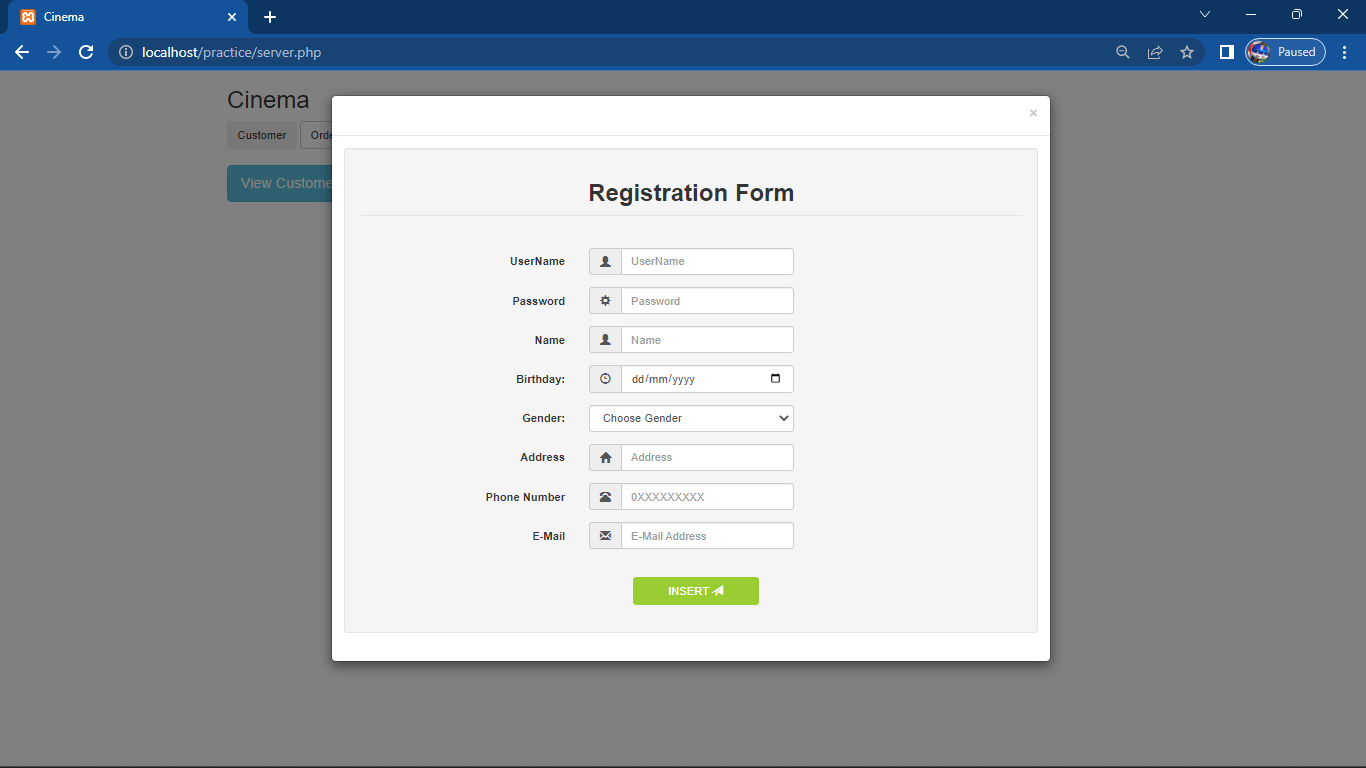
\includegraphics[scale=0.45]{images/insertCustomer.png}
    \caption{Insert Customer}
\end{figure}

Giao diện chứa form cho phép người dùng nhập vào các thông tin của Customer. Ở đây sẽ có validate dữ liệu đầu vào. Ví dụ như format của email, số điện thoại,...

% \subsubsubsection{\textbf{Validate Password}}

\begin{figure}[H]
    \centering
    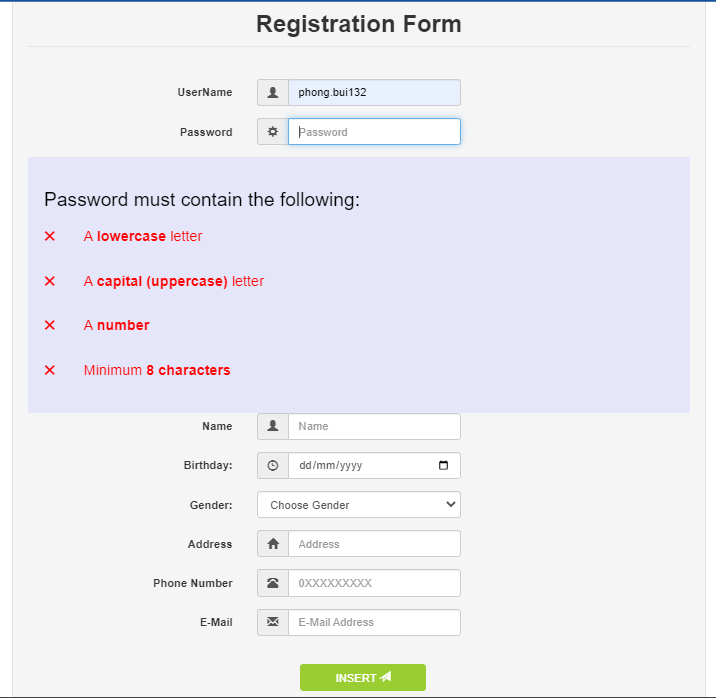
\includegraphics[scale=0.45]{images/insertValidatePassword.png}
    \caption{Validate Password}
\end{figure}
Ở giao diện insert, chúng ta sẽ kiểm tra giá trị nập vào của một số trường. Như ở đây chúng ta kiểm tra giá trị password nhập vào phải chứa cả ký tự in thường, in hoa, số và phải có độ dài hơn từ 8 ký tự trở lên.

\begin{figure}[H]
    \centering
    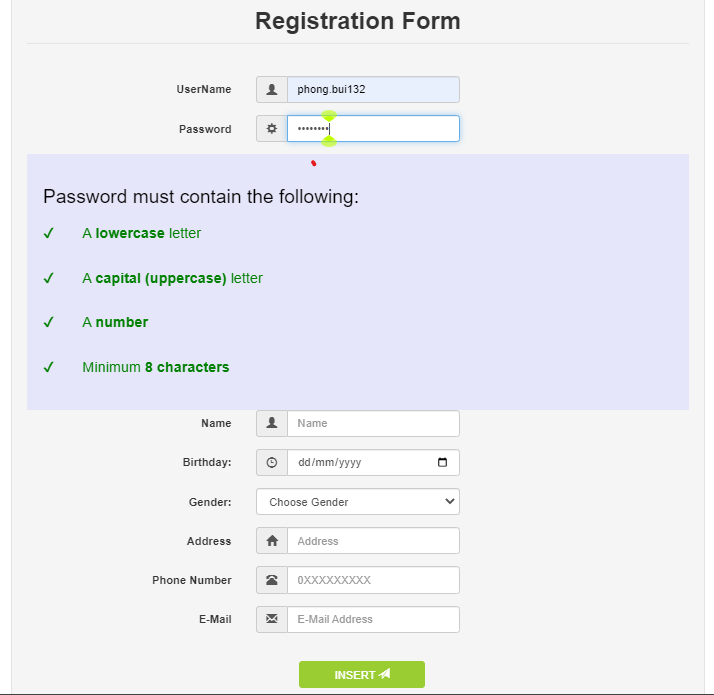
\includegraphics[scale=0.45]{images/insertValidateRightPassword.png}
    \caption{Validate Password}
\end{figure}
Khi input được nhập thì sẽ những điều kiện sẽ hiển thị màu xanh ở những điều kiện thoải mãn.

\begin{figure}[H]
    \centering
    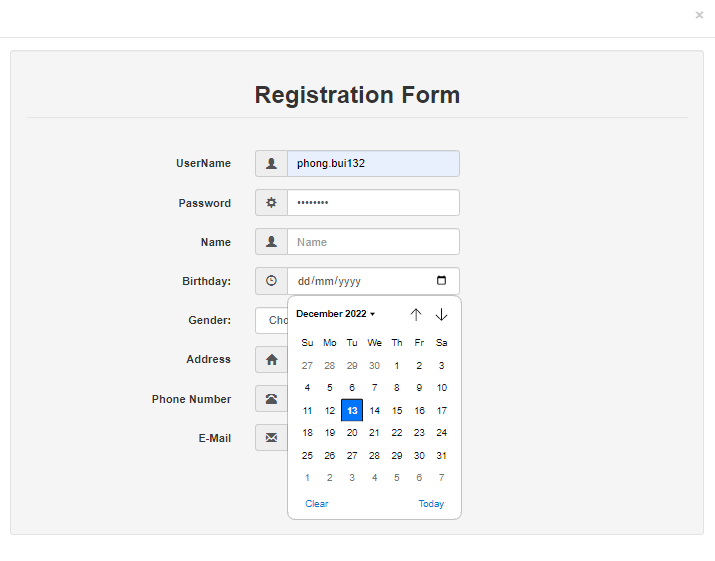
\includegraphics[scale=0.45]{images/calendarPicker.png}
    \caption{Calendar picker}
\end{figure}
Khi chọn vào trường Birthday để nhập thì calendar picker sẽ được hiển thị để người dùng chọn.

\begin{figure}[H]
    \centering
    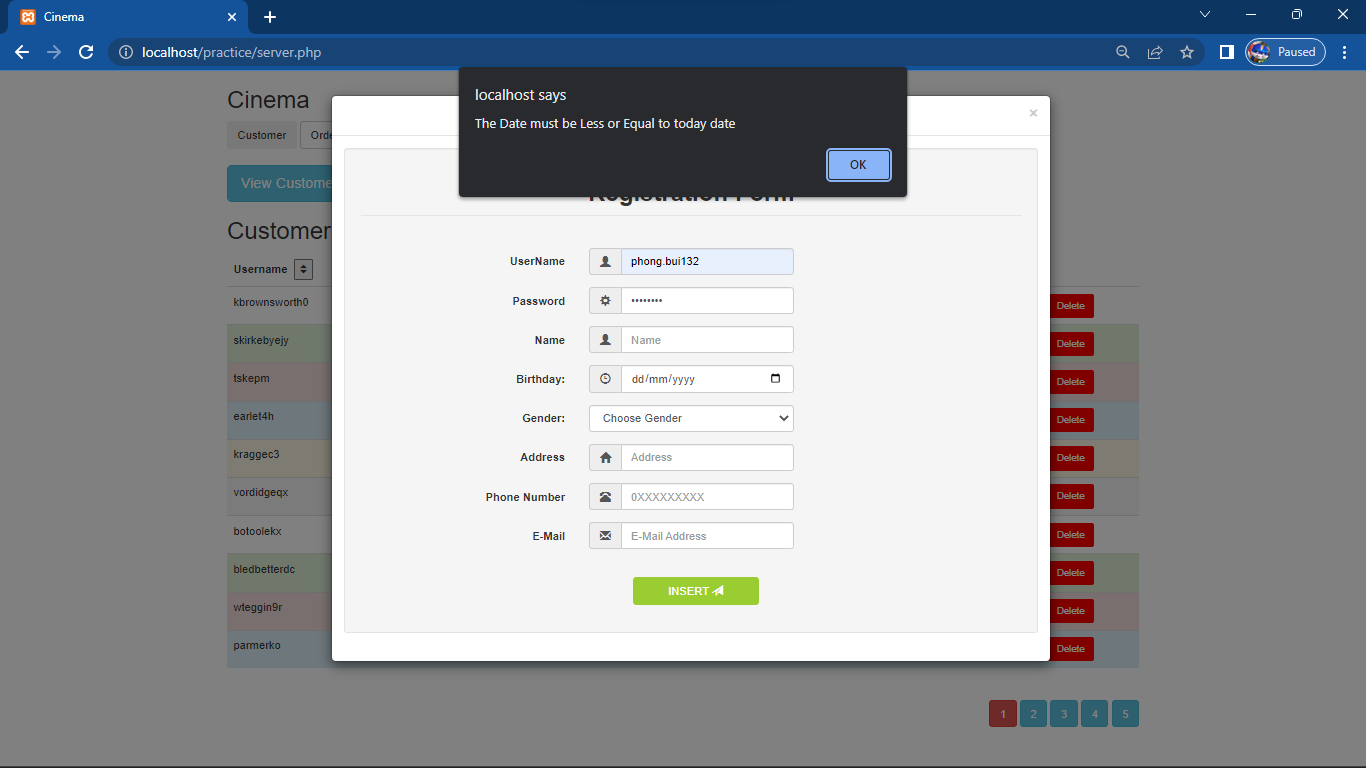
\includegraphics[scale=0.45]{images/validateBirthday.png}
    \caption{Validate Birthday}
\end{figure}
Nếu ngày được chọn lớn hơn ngày ở hiện tại thì sẽ có thông báo được hiện ra về việc input Birthday không hợp lệ.

\begin{figure}[H]
    \centering
    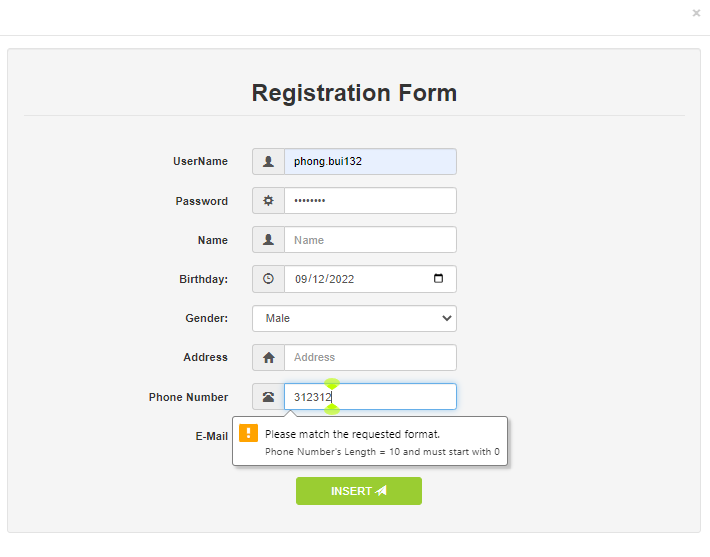
\includegraphics[scale=0.45]{images/validatePhone.png}
    \caption{Validate Phone Number}
\end{figure}
Format được dùng cho Phone Number là phải bắt đầu bằng "0" và độ dài phải là 10 số. Nếu nhập sai sẽ có thông báo hiển thị.

\begin{figure}[H]
    \centering
    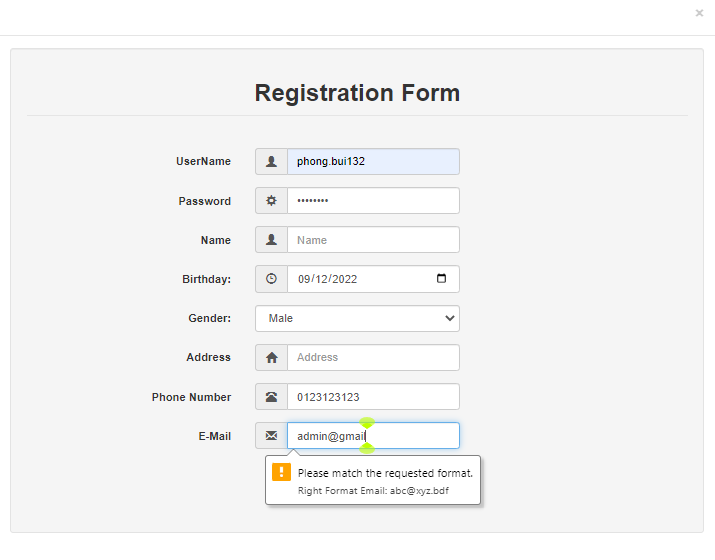
\includegraphics[scale=0.45]{images/validateEmail.png}
    \caption{Validate Email}
\end{figure}
Format của email sẽ là "abc@xyz.bdf". Nếu không có "@" hoặc sau "@xyz." không có thì sẽ báo lỗi.
\begin{figure}[H]
    \centering
    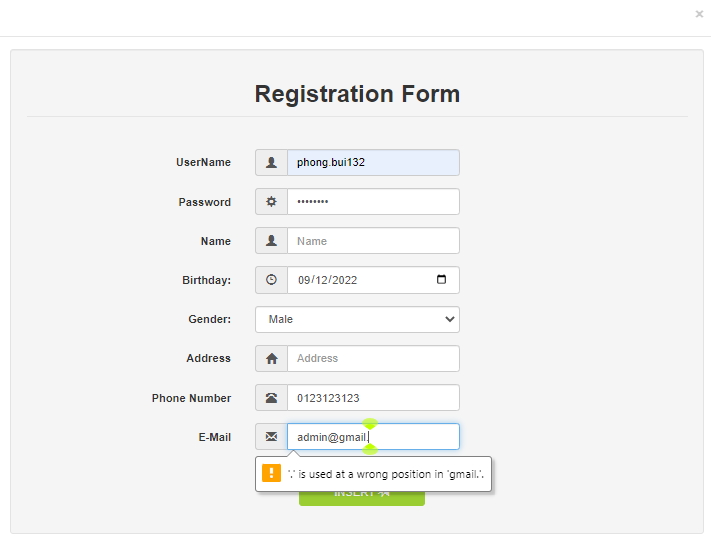
\includegraphics[scale=0.45]{images/validateEmail_02.png}
    \caption{Validate Email}
\end{figure}


\subsubsection{Search Information}
\begin{figure}[H]
    \centering
    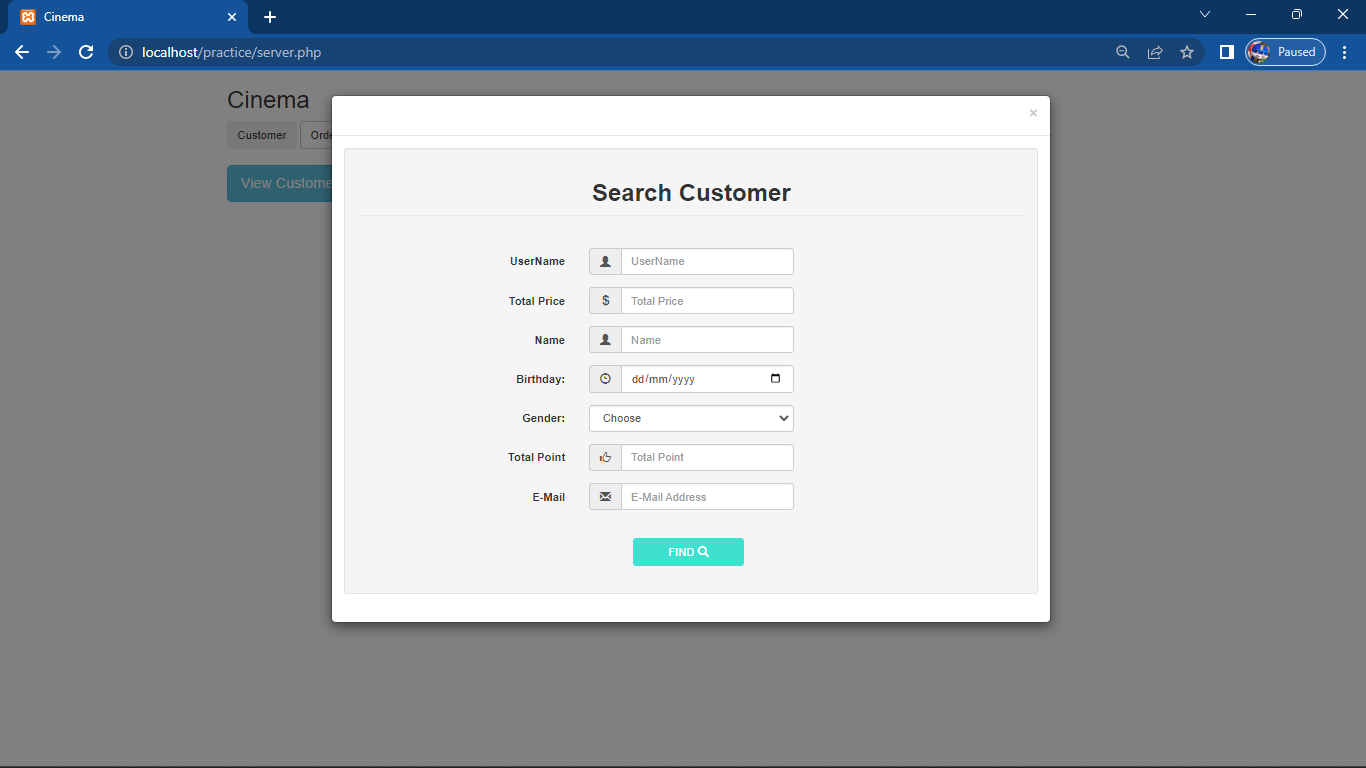
\includegraphics[scale=0.45]{images/searchAndFilter_Customer.png}
    \caption{Search Information About Customer}
\end{figure}
Giao diện chứa form có thể nhập một số thông tin để tìm kiếm. Như muốn tìm kiếm một Customer nào đó chúng ta có thể nhập vào Username hoặc Name hoặc email của họ. Nếu chúng ta chỉ chọn Gender thì kết quả sẽ lọc ra những Customer có giới tính là Gender đã chọn. Nếu nhập vào Total Price thì sẽ lọc ra những Customer có tổng giá trị đơn hàng đã mua từ giá trị đã nhập trở lên.

\subsubsection{Find Order}
\begin{figure}[H]
    \centering
    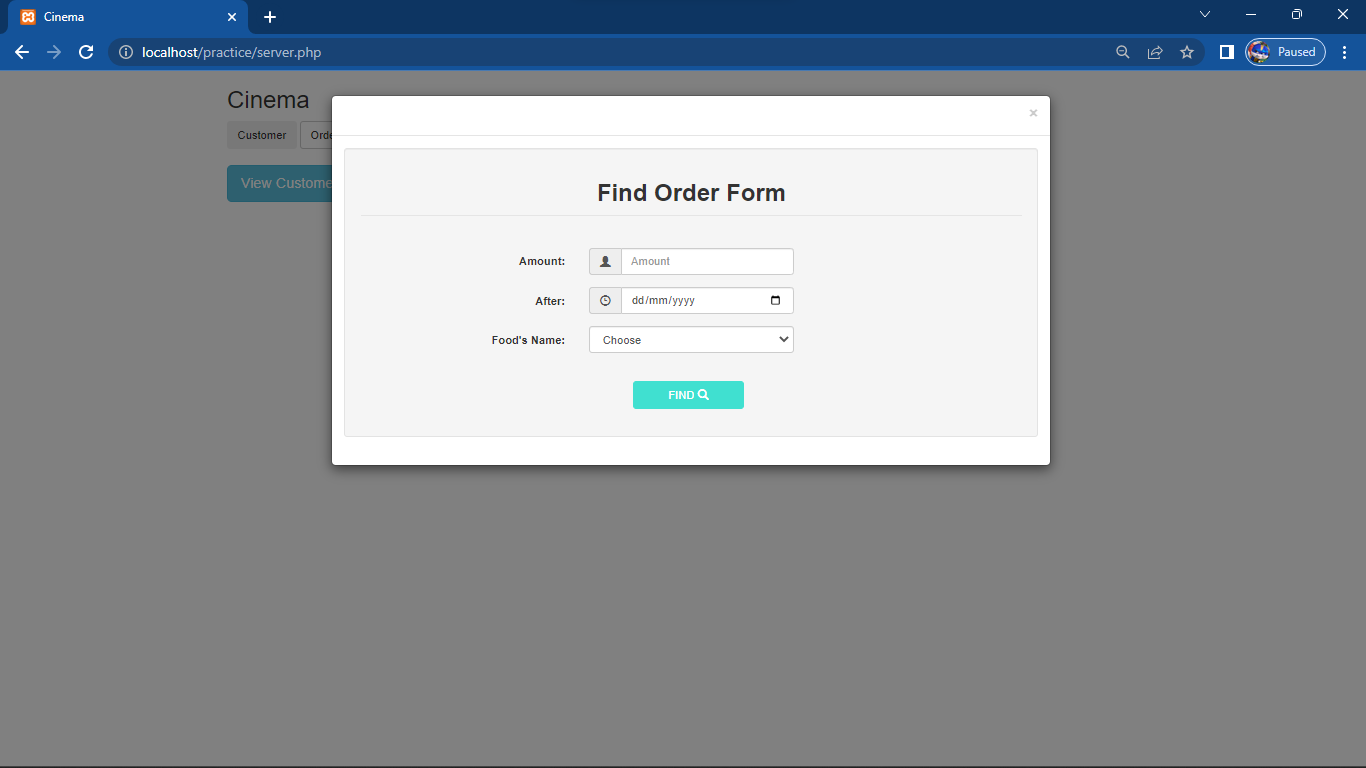
\includegraphics[scale=0.45]{images/findOrder.png}
    \caption{Find Order}
\end{figure}
Giao diện này cho phép chúng ta tìm những đơn hàng Food với một số lượng nhất định sau ngày mà chúng ta đã chọn.


\subsubsection{Find Date Reach Target}
\begin{figure}[H]
    \centering
    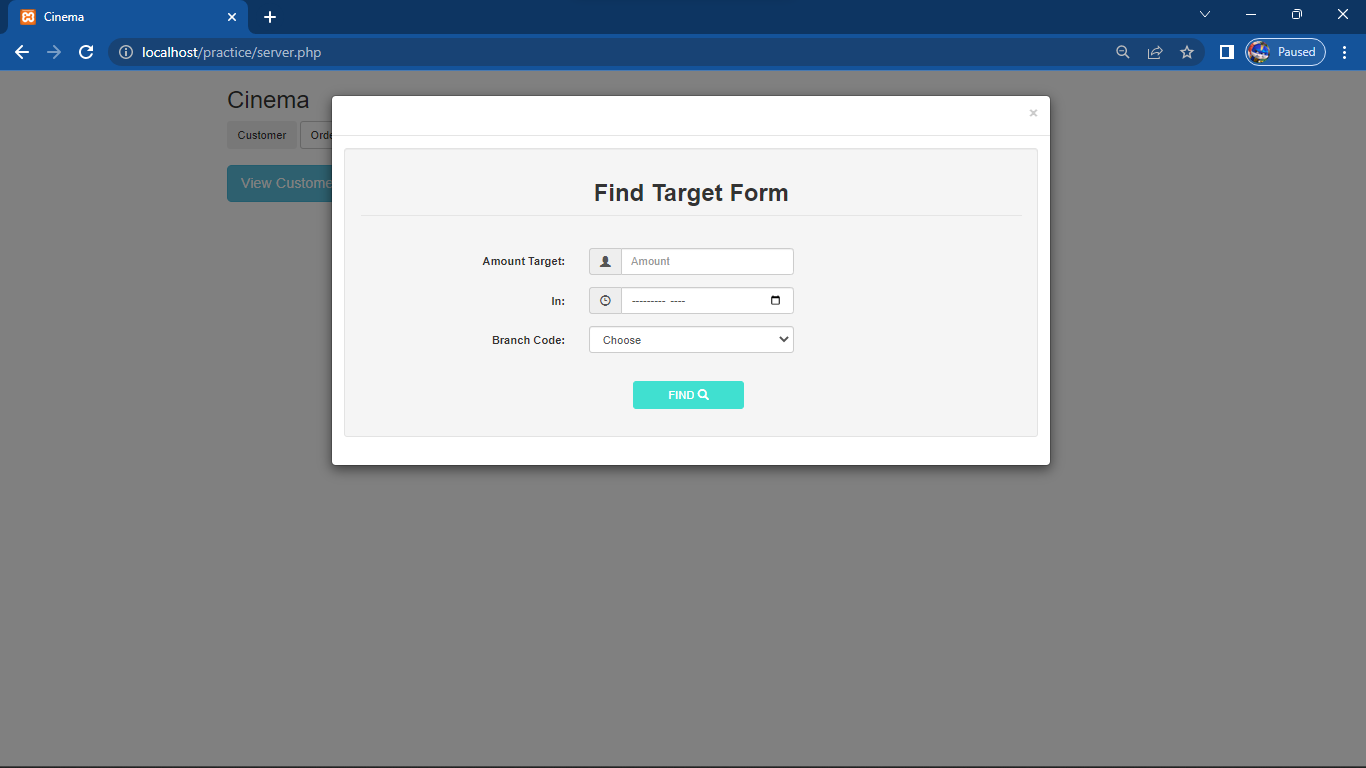
\includegraphics[scale=0.45]{images/findDateReachTarget.png}
    \caption{Find Date Reach Specific Target}
\end{figure}

Giao diện này giúp chúng ta tìm được ngày mà chúng ta đạt doanh thu đề ra trong tháng.


\section*{Phụ lục}
\subsection*{EERD}
\begin{figure}[H]
    \centering
    \href{https://app.diagrams.net/#G1-STSb4oAwxJJz8PLXzsCd5HWxfR61LCN}{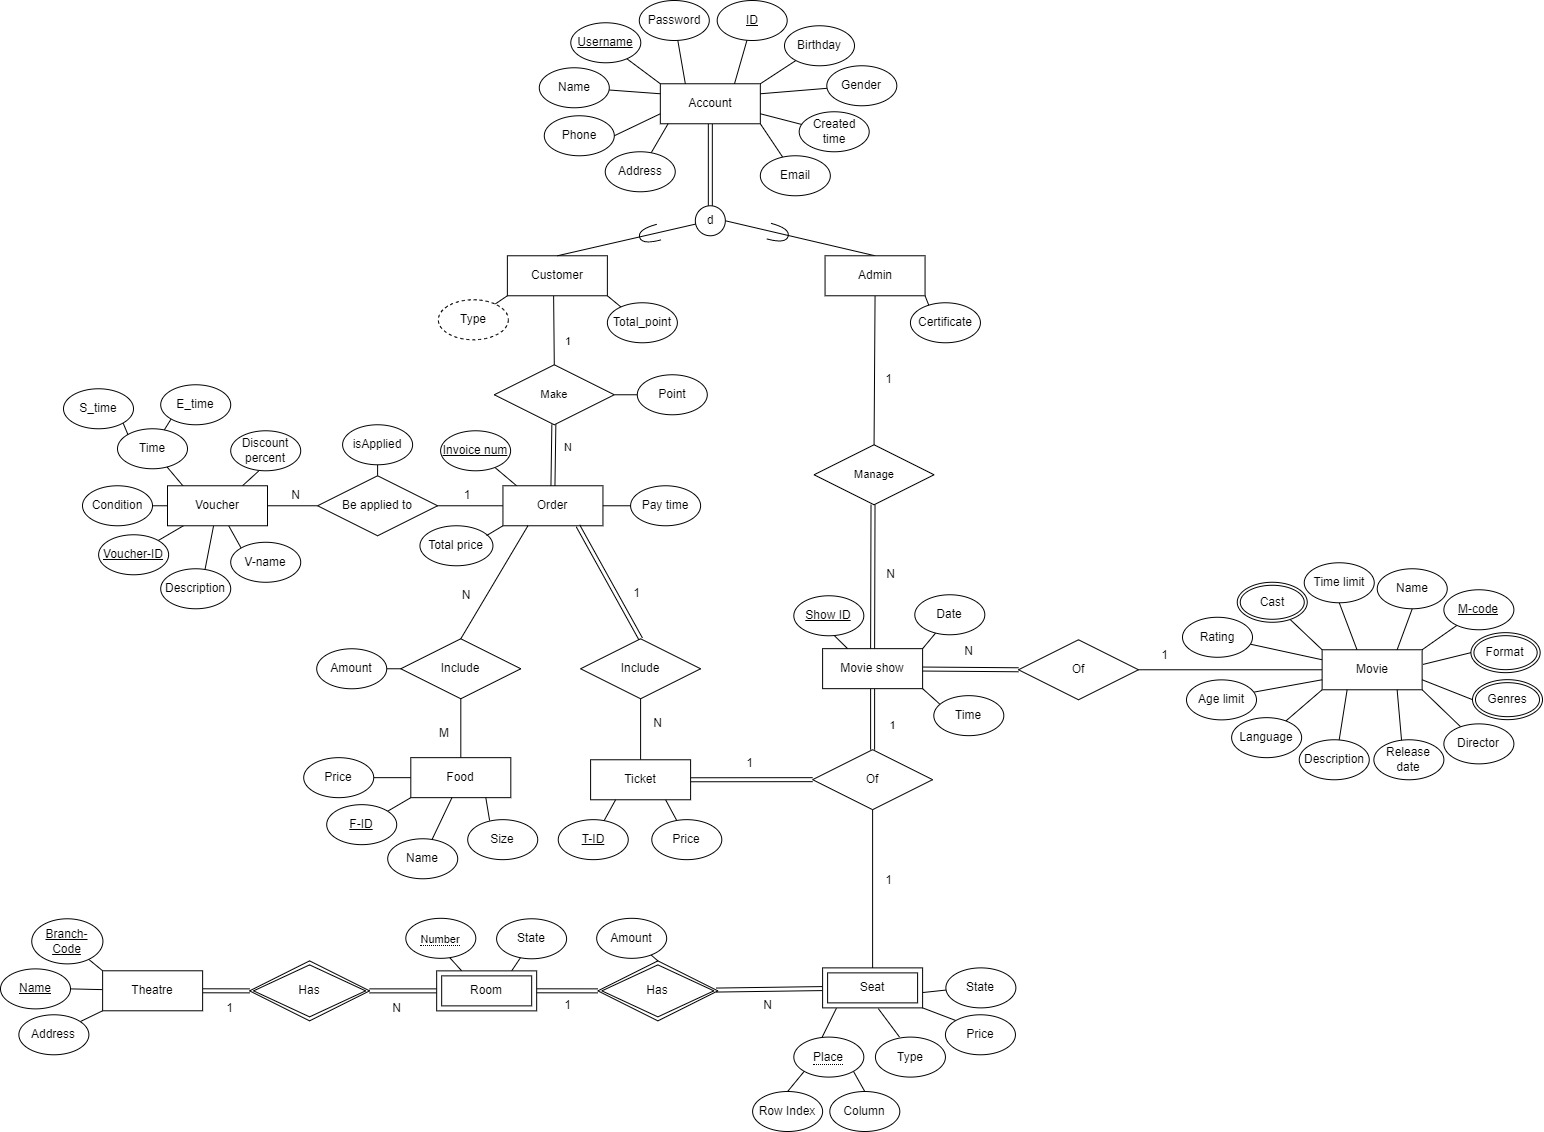
\includegraphics[scale=0.4, angle=270]{images/EERD_E-Cinema.jpg}}
    \caption{E-cinema EERD}
    \label{fig:my_EERD}
\end{figure}


\newpage
%-------------------- references --------------------%
%\begin{thebibliography}{9}
%\bibitem{bib0}
%\href{https://www.youtube.com/watch?v=HSOtku1j600}{Ahihihihihi}
%\end{thebibliography}
\end{document}
